	%%  A simple AAU report template.

%  2014-09-13 v. 1.1.0
%  Copyright 2010-2014 by Jesper Kjær Nielsen <jkn@es.aau.dk>
%
%  This is free software: you can redistribute it and/or modify
%  it under the terms of the GNU General Public License as published by
	%  the Free Software Foundation, either version 3 of the License, or
%  (at your option) any later version.
%
%  This is distributed in the hope that it will be useful,
%  but WITHOUT ANY WARRANTY; without even the implied warranty of
%  MERCHANTABILITY or FITNESS FOR A PARTICULAR PURPOSE.  See the
%  GNU General Public License for more details.
%
%  You can find the GNU General Public License at <http://www.gnu.org/licenses/>.
%
%  A simple AAU report template.
%  2014-09-13 v. 1.1.0
%  Copyright 2010-2014 by Jesper Kjær Nielsen <jkn@es.aau.dk>
%
%  This is free software: you can redistribute it and/or modify
%  it under the terms of the GNU General Public License as published by
%  the Free Software Foundation, either version 3 of the License, or
%  (at your option) any later version.
%
%  This is distributed in the hope that it will be useful,
%  but WITHOUT ANY WARRANTY; without even the implied warranty of
%  MERCHANTABILITY or FITNESS FOR A PARTICULAR PURPOSE.  See the
%  GNU General Public License for more details.
%
%  You can find the GNU General Public License at <http://www.gnu.org/licenses/>.
%
\documentclass[11pt,twoside,a4paper,openright]{report}
%%%%%%%%%%%%%%%%%%%%%%%%%%%%%%%%%%%%%%%%%%%%%%%%
% Language, Encoding and Fonts
% http://en.wikibooks.org/wiki/LaTeX/Internationalization
%%%%%%%%%%%%%%%%%%%%%%%%%%%%%%%%%%%%%%%%%%%%%%%%
% Select encoding of your inputs. Depends on
% your operating system and its default input
% encoding. Typically, you should use
%   Linux  : utf8 (most modern Linux distributions)
%            latin1 
%   Windows: ansinew
%            latin1 (works in most cases)
%   Mac    : applemac
% Notice that you can manually change the input
% encoding of your files by selecting "save as"
% an select the desired input encoding. 
\usepackage[utf8]{inputenc}
% Make latex understand and use the typographic
% rules of the language used in the document.
\usepackage[danish,english]{babel}
% Use the vector font Latin Modern which is going
% to be the default font in latex in the future.
\usepackage{lmodern}
% Choose the font encoding
\usepackage[T1]{fontenc}
% For checkmarks: \cmark and crossmarks: \xmark
\usepackage{pifont}
	\newcommand{\cmark}{\ding{51}}%
	\newcommand{\xmark}{\ding{55}}%
%%%%%%%%%%%%%%%%%%%%%%%%%%%%%%%%%%%%%%%%%%%%%%%%
% Graphics and Tables
% http://en.wikibooks.org/wiki/LaTeX/Importing_Graphics
% http://en.wikibooks.org/wiki/LaTeX/Tables
% http://en.wikibooks.org/wiki/LaTeX/Colors
%%%%%%%%%%%%%%%%%%%%%%%%%%%%%%%%%%%%%%%%%%%%%%%%
% load a colour package
\usepackage[table,dvipsnames]{xcolor}
\definecolor{aaublue}{RGB}{33,26,82}% dark blue
\definecolor{lightGrey}{RGB}{240,240,240}% 
\definecolor{Grey}{gray}{0.7}
% The standard graphics inclusion package
\usepackage{graphicx}
% Load package to convert eps-files to use as figures
\usepackage{epstopdf}

%\usepackage[dvips,final]{graphicx} 
%\usepackage[dvips]{geometry}
\usepackage{color,soul} %include even if images aren’t in color \usepackage{epsfig}
\usepackage{latexsym}
\usepackage{pstricks}

%\usepackage{epsfig}

% Set up how figure and table captions are displayed
\usepackage{caption}
\captionsetup{%
  font=footnotesize,% set font size to footnotesize
  labelfont=bf % bold label (e.g., Figure 3.2) font
}
\usepackage[section]{placeins} % Figurer overskrider ikke sections
% For subfigures
\usepackage{subcaption}
% Make the standard latex tables look so much better
\usepackage{array,booktabs}
% Enable the use of frames around, e.g., theorems
% The framed package is used in the example environment
\usepackage{framed}

% Afstand mellem listepunkter og tilføjelse af resume funktion til lister: \begin{enumerate}[resume]
\usepackage{enumitem}
\setlist{itemsep=-2pt}

% Tilføjer mulighed for at lave enkelte sider i landskab.
\usepackage{lscape}

\newcounter{listcounter}
%%%%%%%%%%%%%%%%%%%%%%%%%%%%%%%%%%%%%%%%%%%%%%%%
% Mathematics
% http://en.wikibooks.org/wiki/LaTeX/Mathematics
%%%%%%%%%%%%%%%%%%%%%%%%%%%%%%%%%%%%%%%%%%%%%%%%
% Defines new environments such as equation,
% align and split 
\usepackage{amsmath}
% Adds new math symbols
\usepackage{amssymb}
% Use theorems in your document
% The ntheorem package is also used for the example environment
% When using thmmarks, amsmath must be an option as well. Otherwise \eqref doesn't work anymore.
\usepackage[framed,amsmath,thmmarks]{ntheorem}

% Tilføjer \degree symbol
\usepackage{textcomp}
\usepackage{gensymb}

% Fjerner mellemrum efter komma i formler.
%\usepackage{icomma}

% Packages for SI units
\usepackage[binary-units]{siunitx}
% Format SI units as italic in italic texts
\sisetup{detect-all}
\sisetup{per-mode=symbol}


% Argument til amsmath der gør parenteser uden om parenteser pænere ved brug af \right og \left kommandoerne
\delimitershortfall=-1pt

%%%%%%%%%%%%%%%%%%%%%%%%%%%%%%%%%%%%%%%%%%%%%%%%
% Page Layout
% http://en.wikibooks.org/wiki/LaTeX/Page_Layout
%%%%%%%%%%%%%%%%%%%%%%%%%%%%%%%%%%%%%%%%%%%%%%%%
% Change margins, papersize, etc of the document
\usepackage[
  inner=28mm,% left margin on an odd page
  outer=41mm,% right margin on an odd page
  ]{geometry}
% Modify how \chapter, \section, etc. look
% The titlesec package is very configureable
\usepackage[explicit]{titlesec}
%\titleformat*{\section}{\normalfont\Large\bfseries\color{aaublue}}
%\titleformat*{\subsection}{\normalfont\large\bfseries\color{aaublue}}
%\titleformat*{\subsubsection}{\normalfont\normalsize\bfseries\color{aaublue}}
%\titleformat*{\paragraph}{\normalfont\normalsize\bfseries\color{aaublue}}
%\titleformat*{\subparagraph}{\normalfont\normalsize\bfseries\color{aaublue}}
\usepackage{calc}

% Spacing omkring kapiteloverskrift
\titlespacing*{\chapter}{0pt}{40pt}{50pt}



% Overskrift med stort nummer til venstre og titel til højre
%\newlength\chapnumb
%\setlength{\chapnumb}{1.5cm}
%\titleformat{\chapter}[block]
%{\normalfont\bfseries}{}{0pt}
%{\parbox[b]{\chapnumb}{%
	  %\fontsize{2cm}{0}\selectfont\thechapter}%
  %\parbox[b]{\dimexpr\textwidth-\chapnumb\relax}{%
    %\raggedleft%
    %\hfill{\Huge#1}\\
    %\rule{\dimexpr\textwidth-\chapnumb\relax}{.5pt}}}
%\titleformat{name=\chapter,numberless}[block]
%{\normalfont\bfseries}{}{0pt}
	%{\Huge#1}

% Clear empty pages between chapters
\let\origdoublepage\cleardoublepage
\newcommand{\clearemptydoublepage}{%
  \clearpage
  {\pagestyle{empty}\origdoublepage}%
}
\let\cleardoublepage\clearemptydoublepage

% Change the headers and footers
\usepackage{fancyhdr}
\pagestyle{fancy}
\fancyhf{} %delete everything
\renewcommand{\headrulewidth}{0pt} %remove the horizontal line in the header
\fancyhead[RE]{\color{black}\small\nouppercase\leftmark} %even page - chapter title
\fancyhead[LO]{\color{black}\small\nouppercase\rightmark} %uneven page - section title
\fancyhead[LE,RO]{\thepage} %page number on all pages
% Do not stretch the content of a page. Instead,
% insert white space at the bottom of the page
\raggedbottom
% Enable arithmetics with length. Useful when
% typesetting the layout.

\setlength{\headheight}{10pt}

% Raise penalties for bastards
\widowpenalty=10000
\clubpenalty=10000

%%%%%%%%%%%%%%%%%%%%%%%%%%%%%%%%%%%%%%%%%%%%%%%%
% Table of Contents
% http://en.wikibooks.org/wiki/LaTeX/Bibliography_Management
%%%%%%%%%%%%%%%%%%%%%%%%%%%%%%%%%%%%%%%%%%%%%%%%
% Add additional commands for Table of Contents
\usepackage{bookmark}

{\setcounter{tocdepth}{1}}

% Control of space between items in Table of Contents
\usepackage[titles]{tocloft}
\setlength{\cftbeforepartskip}{10pt}
\setlength{\cftbeforechapskip}{4pt}
\setlength{\cftbeforesecskip}{2pt}
%%%%%%%%%%%%%%%%%%%%%%%%%%%%%%%%%%%%%%%%%%%%%%%%
% Bibliography
% http://en.wikibooks.org/wiki/LaTeX/Bibliography_Management
%%%%%%%%%%%%%%%%%%%%%%%%%%%%%%%%%%%%%%%%%%%%%%%%
% Add the \citep{key} command which display a
% reference as [author, year]
\usepackage[square]{natbib}

%%%%%%%%%%%%%%%%%%%%%%%%%%%%%%%%%%%%%%%%%%%%%%%%
% Misc
%%%%%%%%%%%%%%%%%%%%%%%%%%%%%%%%%%%%%%%%%%%%%%%%
% Add bibliography and index to the table of
% contents
\usepackage[nottoc]{tocbibind}
% Add the command \pageref{LastPage} which refers to the
% page number of the last page
\usepackage{lastpage}
\usepackage[
%  disable, %turn off todonotes
  colorinlistoftodos, %enable a coloured square in the list of todos
  textwidth=\marginparwidth, %set the width of the todonotes
  textsize=scriptsize, %size of the text in the todonotes
  ]{todonotes}

% Add command \includepdf to add a whole pdf page to document
\usepackage{pdfpages}


% Add option to easy format directory tree
\usepackage{dirtree}

% String manipulation
\usepackage{xstring,xifthen}

% Tikz package for drawing nice figures
\usepackage{tikz}
\usepackage{schemabloc}
\usetikzlibrary{circuits}


% Package for drawing pretty schematics, without leaving LaTex
\usepackage[american currents, american voltages, european resistors, cute inductors,
american ports]{circuitikz}
\usepackage{tikzscale}

% Code syntax highlight
\usepackage{listings}
\lstset{breaklines=true,
		breakatwhitespace=true,
		commentstyle=\color{ForestGreen},
		numbers=left,
		numberstyle=\tiny\color{black},
		keywordstyle=\color{blue},
		basicstyle=\footnotesize\ttfamily,
        showstringspaces=false,
		}
\renewcommand{\lstlistingname}{Code Snippet}

%%%%%%%%%%%%%%%%%%%%%%%%%%%%%%%%%%%%%%%%%%%%%%%%
% Table environments
% http://en.wikibooks.org/wiki/LaTeX/Tables
%%%%%%%%%%%%%%%%%%%%%%%%%%%%%%%%%%%%%%%%%%%%%%%%
% Better table environments for stuff like table width specifier
\usepackage{tabularx}
\usepackage{multirow}
\usepackage{longtable}
\usepackage{makecell}
%%%%%%%%%%%%%%%%%%%%%%%%%%%%%%%%%%%%%%%%%%%%%%%%
% Project info and abstract
% chapters\abstract.tex, chapters\projectinfo.tex
%%%%%%%%%%%%%%%%%%%%%%%%%%%%%%%%%%%%%%%%%%%%%%%%
% Loads project info and abstract for use in
% hypersetup
\newcommand{\projectFaculty}{%
\iflanguage{english}{%
Vision, Graphics and Interactive Systems%
}{%
Vision, Grafik og Interaktive Systemer%
}}

\newcommand{\projectGroup}{%
\iflanguage{english}{%
VGIS10 Group 1043%
}{%
Niclas Hjorth Stjernholm%
}}

\newcommand{\projectSemester}{%
VGIS10%
}

\newcommand{\projectType}{%
\iflanguage{english}{%
Master Thesis%
}{%
Projektrapport%
}}

\newcommand{\projectTitle}{%
\iflanguage{english}{%
Zebrafish Occlusion Detection%
}{%
Noget med Computer Vision%
}}

\newcommand{\projectSubtitle}{%
\iflanguage{english}{%
- Subtitle -%
}{%
- Undertitel -%
}}

\newcommand{\projectTheme}{%
\iflanguage{english}{%
Computer Vision%
}{%
Computer Vision%
}}

\newcommand{\projectPeriod}{%
\iflanguage{english}{%
Spring Semester 2019%
}{%
Forårssemester 2018%
}}



\newcommand{\projectParticipants}{%
Niclas Hjorth Stjernholm
}

\newcommand{\projectSupervisors}{%
Malte Pedersen\\
Thomas B. Moeslund
}

\newcommand{\projectCopies}{8}

\newcommand{\projectCompletion}{
\iflanguage{english}{%
October 11, 2019%
}{
30. maj 2018%
}}

\newcommand{\projectAbstract}{

}

\newcommand{\projectSynopsis}{
Synopsis
}


%%%%%%%%%%%%%%%%%%%%%%%%%%%%%%%%%%%%%%%%%%%%%%%%
% Hyperlinks
% http://en.wikibooks.org/wiki/LaTeX/Hyperlinks
%%%%%%%%%%%%%%%%%%%%%%%%%%%%%%%%%%%%%%%%%%%%%%%%
% Enable hyperlinks and insert info into the pdf
% file. Hypperref should be loaded as one of the 
% last packages
\usepackage{hyperref}
\hypersetup{%
	%pdfpagelabels=true,%
	plainpages=false,%
	pdfauthor={\projectGroup, \projectFaculty, \iflanguage{english}{Aalborg University}{Aalborg Universitet}},%
	pdftitle={\projectTitle},%
	pdfsubject={\projectTheme},%
	bookmarksnumbered=true,%
	colorlinks,%
	citecolor=black,%aaublue,%
	filecolor=black,%aaublue,%
	linkcolor=black,%aaublue,% you should probably change this to black before printing
	urlcolor=black,%aaublue,%
	pdfstartview=FitH,%
	bookmarksdepth=2,%
}

% Defines where URLs should break
\def\UrlBreaks{\do\/\do-\do_}
\urlstyle{same}

% Give the possibility to autoformat reference based on distance to the referenced page. Ex. \vpageref{}
\usepackage{varioref}


% Package to warn about missing references.
%\usepackage{refcheck}

% Package to make a glossary of acronyms.
\usepackage[nonumberlist]{glossaries}
\usepackage{glossary-mcols}
\glstoctrue
\makenoidxglossaries
\glssetwidest{DeepID2  }
\glossarystyle{alttree}
% Glossaries package
% http://ctan.cs.uu.nl/macros/latex/contrib/glossaries/glossariesbegin.pdf
%
% % % % % % % %
%	Example of glossary entry:
% \newglossaryentry{cabbage}{name={cabbage},description={vegetable with thick green or purple leaves}}
%
%	Example of acronym entry:
% \newacronym{spi}{SPI}{Serial Peripheral Interface}
%
% \gls{key}

\newacronym{cdf}{CDF}{Cumulative Distribution Function}
\newacronym{cnn}{CNN}{Convolutional Neural Network}
\newacronym{cpu}{CPU}{Central Processing Unit}
\newacronym{fcn}{FCN}{Fully Convolutional Network}
\newacronym{dbn}{DBN}{Deep Belief Network}
\newacronym{deepid}{DeepID}{Deep hidden identity features}
\newacronym{deepid2}{DeepID2}{Deep IDentification-verification features}
\newacronym{gpu}{GPU}{Graphics Processing Unit}
\newacronym{spdnn}{SPDNN}{Semi Parallel Deep Neural Networks}
\newacronym{lfw}{LFW}{Labeled Faces in the Wild}
\newacronym{hmm}{HMM}{Hidden Markov Model}
\newacronym{lda}{LDA}{Linear Discriminant Analysis}
\newacronym{pca}{PCA}{Principal Component Analysis}
\newacronym{svm}{SVM}{support vector machines}
\newacronym{knn}{KNN}{K-Nearest-Neighbours}
\newacronym{vl}{VL}{Visible Light}
\newacronym{nir}{NIR}{Near Infra-Red}
\newacronym{mcs}{MCS}{Multiple Classifier Systems}
\newacronym{relu}{ReLU}{Rectified Linear Unit}
\newacronym{fc}{FC}{Fully Connected}
\newacronym{yolo}{YOLO}{You Only Look Once}
\newacronym{doh}{DoH}{Determinant of Hessian}
\newacronym{blob}{BLOB}{Binary Large Object}
\newacronym{roi}{ROI}{Region of Interest}
\newacronym{surf}{SURF}{Speeded-Up Robust Features}
\newacronym{fps}{FPS}{Frames Per Second}
\newacronym{map}{mAP}{mean Average Precision}
\newacronym{iou}{IoU}{Intersection over Union}
\newacronym{rcnn}{R-CNN}{Region-based Convolutional Neural Network}
\newacronym{coco}{COCO}{Common Objects in Context}

% Package to make semi-bold font.
\usepackage[outline]{contour}
\contourlength{0.1pt}
\contournumber{50}%
\newcommand{\textsb}[1]{\contour{black}{#1}}

% Package for splitting lists or other things up in columns. Ex: \begin{multicols}{2}
\usepackage{multicol}

% Package for rotating a page to landscape orientation. Ex: \begin{landscape}
\usepackage{pdflscape}

% Package for circuit diagrams in tikz
\usepackage{circuitikz}

% For adding notes to tables
\usepackage{threeparttable}

% For adding smileys ;) I know....
\usepackage{MnSymbol,wasysym}

% For adding algorithms
\usepackage{algorithm}
\usepackage[noend]{algpseudocode}
\makeatletter
\def\BState{\State\hskip-\ALG@thistlm}
\makeatother

\renewcommand*{\glsgroupskip}{\vspace{2mm}}

% Package to use fixme fxnote
\usepackage[footnote,marginclue,draft,danish,silent,nomargin]{fixme} 

% Package inclusion and set up of the document

% see, e.g., http://en.wikibooks.org/wiki/LaTeX/Formatting#Hyphenation
% for more information on word hyphenation
\hyphenation{ex-am-ple hy-phen-a-tion short}
\hyphenation{long la-tex}
\hyphenation{AAU-Sat}
\hyphenation{minimum-spændinger}
\hyphenation{ud-vik-lings-poten-tiale}
\hyphenation{pick-up pick-up-pen gui-tar-pick-up gui-tar-pick-up-pen pick-uppens}
\hyphenation{tech-no-lo-gy}
\hyphenation{Hø-re-for-e-ning-en}
\hyphenation{dis-cri-mi-nant}% Hypenation setup

%  A simple AAU report template.
%  2014-09-13 v. 1.1.0
%  Copyright 2010-2014 by Jesper Kjær Nielsen <jkn@es.aau.dk>
%
%  This is free software: you can redistribute it and/or modify
%  it under the terms of the GNU General Public License as published by
%  the Free Software Foundation, either version 3 of the License, or
%  (at your option) any later version.
%
%  This is distributed in the hope that it will be useful,
%  but WITHOUT ANY WARRANTY; without even the implied warranty of
%  MERCHANTABILITY or FITNESS FOR A PARTICULAR PURPOSE.  See the
%  GNU General Public License for more details.
%
%  You can find the GNU General Public License at <http://www.gnu.org/licenses/>.
%
%
%
% see, e.g., http://en.wikibooks.org/wiki/LaTeX/Customizing_LaTeX#New_commands
% for more information on how to create macros

%%%%%%%%%%%%%%%%%%%%%%%%%%%%%%%%%%%%%%%%%%%%%%%%
% Loads user defined variables
%%%%%%%%%%%%%%%%%%%%%%%%%%%%%%%%%%%%%%%%%%%%%%%%

\newcommand{\noSIunit}{$1$}% Definerer hvad der skal skrives hvis symbolet ikke har nogen enhed.
\newcommand{\obcTransducerAddress}{0xB1}% CAN adresse til tranducer modulet i OBC.

\def\circuitScale{.5}%

%%%%%%%%%%%%%%%%%%%%%%%%%%%%%%%%%%%%%%%%%%%%%%%%
% Macros for the titlepage
%%%%%%%%%%%%%%%%%%%%%%%%%%%%%%%%%%%%%%%%%%%%%%%%
%Creates the aau titlepage
\newcommand{\aautitlepage}[3]{%
  {
    %set up various length
    \ifx\titlepageleftcolumnwidth\undefined
      \newlength{\titlepageleftcolumnwidth}
      \newlength{\titlepagerightcolumnwidth}
    \fi
    \setlength{\titlepageleftcolumnwidth}{0.5\textwidth-\tabcolsep}
    \setlength{\titlepagerightcolumnwidth}{\textwidth-2\tabcolsep-\titlepageleftcolumnwidth}
    %create title page
    \thispagestyle{empty}
    \noindent%
    \begin{tabular}{@{}ll@{}}
      \parbox{\titlepageleftcolumnwidth}{
        \iflanguage{danish}{%
          
\includegraphics[page=1,width=\titlepageleftcolumnwidth]{figures/aau_logo}
        }{%
          
\includegraphics[page=2,width=\titlepageleftcolumnwidth]{figures/aau_logo}
        }
      } &
      \parbox{\titlepagerightcolumnwidth}{\raggedleft\sf\small
        #2
      }\bigskip\\
       #1 &
      \parbox[t]{\titlepagerightcolumnwidth}{%
        \iflanguage{danish}{%
          \textbf{Synopsis:}\smallskip\par
        }{%
          \textbf{Abstract:}\smallskip\par
        }
        \fbox{\parbox{\titlepagerightcolumnwidth-2\fboxsep-2\fboxrule}{%
          #3
        }}
      }\\
    \end{tabular}
    %\vfill
    \iflanguage{danish}{%
      \noindent{\footnotesize\emph{Rapportens indhold er frit tilgængeligt, men offentliggørelse (med kildeangivelse) må kun ske efter aftale med forfatterne.}}
    }{%
      \noindent{\footnotesize\emph{The content of this report is freely available, but publication may only be pursued with reference.}}
    }
    \cleardoublepage
  }
}

%Create english project info
\newcommand{\englishprojectinfo}[8]{%
  \parbox[t]{\titlepageleftcolumnwidth}{
    \textbf{Title:}\\ #1\bigskip\par
    \textbf{Theme:}\\ #2\bigskip\par
    \textbf{Project Period:}\\ #3\bigskip\par
    \textbf{Project Group:}\\ #4\bigskip\par
    \textbf{Participants:}\\ #5\bigskip\par
    \textbf{Supervisor:}\\ #6\bigskip\par
    \textbf{Number of Pages:} \pageref{LastPage}\bigskip\par
    \textbf{Date of Completion:}\\ #8
  }
}

%Create danish project info
\newcommand{\danishprojectinfo}[8]{%
  \parbox[t]{\titlepageleftcolumnwidth}{
    \textbf{Titel:}\\ #1\bigskip\par
    \textbf{Tema:}\\ #2\bigskip\par
    \textbf{Projektperiode:}\\ #3\bigskip\par
    \textbf{Projektgruppe:}\\ #4\bigskip\par
    \textbf{Deltagere:}\\ #5\bigskip\par
    \textbf{Vejleder:}\\ #6\bigskip\par
    \textbf{Oplagstal:} #7\bigskip\par
    \textbf{Sidetal:} \pageref{LastPage}\bigskip\par
    \textbf{Afleveringsdato:}\\ #8
  }
}

%%%%%%%%%%%%%%%%%%%%%%%%%%%%%%%%%%%%%%%%%%%%%%%%
% An example environment
%%%%%%%%%%%%%%%%%%%%%%%%%%%%%%%%%%%%%%%%%%%%%%%%
\theoremheaderfont{\normalfont\bfseries}
\theorembodyfont{\normalfont}
\theoremstyle{break}
\def\theoremframecommand{{\color{aaublue!50}\vrule width 5pt \hspace{5pt}}}
\newshadedtheorem{exa}{Example}[chapter]
\newenvironment{example}[1]{%
		\begin{exa}[#1]
}{%
		\end{exa}
}


%%%%%%%%%%%%%%%%%%%%%%%%%%%%%%%%%%%%%%%%%%%%%%%%%
% Exponential function defined as upright e, \exp
%%%%%%%%%%%%%%%%%%%%%%%%%%%%%%%%%%%%%%%%%%%%%%%%%
\renewcommand{\exp}{\text{e}}


%%%%%%%%%%%%%%%%%%%%%%%%%%%%%%%%%%%%%%%%%%%%%%%%%%%
% Command \clearevenpage start chapter on even page
%%%%%%%%%%%%%%%%%%%%%%%%%%%%%%%%%%%%%%%%%%%%%%%%%%%
\makeatletter
\newcommand*{\clearevenpage}{%
  \clearpage
  \if@twoside
    \ifodd\c@page
      \hbox{}%
      \newpage
      \if@twocolumn
        \hbox{}%
        \newpage
      \fi
    \fi
  \fi
}
\makeatother

%%%%%%%%%%%%%%%%%%%%%%%%%%%%%%%%%%%%%%%%%%%%%%%%%%%%%%%
% Command \addunit. Use it to add si units to equations
%%%%%%%%%%%%%%%%%%%%%%%%%%%%%%%%%%%%%%%%%%%%%%%%%%%%%%%
\makeatletter
\providecommand\add@text{}
\newcommand\addunit[1]{%
  \gdef\add@text{\text{[}\ifthenelse{\equal{#1}{}}{\noSIunit}{\si{#1}}\text{]}\gdef\add@text{}}}% 
\renewcommand\tagform@[1]{%
  \maketag@@@{\llap{\add@text\quad}(\ignorespaces#1\unskip\@@italiccorr)}%
}
\makeatother

%%%%%%%%%%%%%%%%%%%%%%%%%%%%%%%%%%%%%%%%%%%%%
% Oversættelser af ord ved brug af \autoref{}
%%%%%%%%%%%%%%%%%%%%%%%%%%%%%%%%%%%%%%%%%%%%%
\addto\extrasdanish{%
  \def\figureautorefname{Figur}%
  \def\subfigureautorefname{Figur}%
  \def\tableautorefname{Tabel}%
  \def\partautorefname{Del}%
  \def\appendixautorefname{Bilag}%
  \def\equationautorefname{Ligning}%
  \def\Itemautorefname{Punkt}%
  \def\chapterautorefname{Kapitel}%
  \def\sectionautorefname{Afsnit}%
  \def\subsectionautorefname{Afsnit}%
  \def\subsubsectionautorefname{Underafsnit}%
  \def\paragraphautorefname{Delafsnit}%
  \def\Hfootnoteautorefname{Fodnote}%
  \def\AMSautorefname{Ligning}%
  \def\theoremautorefname{Sætning}%
  \def\pageautorefname{Side}%
  \def\requirementautorefname{Krav}%
}

\addto\extrasenglish{%
  \def\sectionautorefname{section}%
  \def\subsectionautorefname{section}%
  \def\subsubsectionautorefname{section}%
  \def\requirementautorefname{Requirement}%
  \def\algorithmautorefname{Algorithm}%
}

%%%%%%%%%%%%%%%%%%%%%%%%%%%%%%%%%%%%%%%%%%%%%%%%%%%%%%%%%%%%%%%%%%%%%%
% Tilføjer kommando \fullref{} for både at referere til nummer og navn
%%%%%%%%%%%%%%%%%%%%%%%%%%%%%%%%%%%%%%%%%%%%%%%%%%%%%%%%%%%%%%%%%%%%%%
\renewcommand*{\fullref}[1]{\hyperref[{#1}]{\autoref*{#1} \nameref*{#1}}} % One single link


%%%%%%%%%%%%%%%%%%%%%%%%%%%%%%%%%%%%%%%%%%%%%%%%%%%%%%%%%%%%%%%%%%%%%%
% Tilføjer forkortelser af ord.
%%%%%%%%%%%%%%%%%%%%%%%%%%%%%%%%%%%%%%%%%%%%%%%%%%%%%%%%%%%%%%%%%%%%%%
\newcommand{\AAU}{%
\iflanguage{english}{%
Aalborg University%
}{%
Aalborg Universitet%
}}

\newcommand{\opamp}{%
\iflanguage{english}{%
operational amplifier%
}{%
operationsforstærker%
}}

\newcommand{\hifi}{%
\iflanguage{english}{%
hi-fi amplifier%
}{%
hi-fi-forstærker%
}}

%%%%%%%%%%%%%%%%%%%%%%%%%%%%%%%%%%%%%%%%%%%%%%%%%%%%%%%%%%%%%%%%%%%%%%
% Command \DefVar{VARIBLE_NAME}
% Is used to create a variable.
% Set varible: \VARIBLE_NAME{VALUE}
% Get varible: \getVARIBLE_NAME
%%%%%%%%%%%%%%%%%%%%%%%%%%%%%%%%%%%%%%%%%%%%%%%%%%%%%%%%%%%%%%%%%%%%%%

\makeatletter%
\newcommand{\DefVar}[1]{\@namedef{#1}##1{\global\@namedef{get#1}{##1}}\@nameuse{#1}{}}%
\makeatother%

%%%%%%%%%%%%%%%%%%%%%%%%%%%%%%%%%%%%%%%%%%%%%%%%%%%%%%%%%%%%%%%%%%%%%%
% Requirements environment:
%
% \begin{requirement}
%   \requirement{}
%   \argument{}
%   \fullfilment{}
% \end{requirement}
%%%%%%%%%%%%%%%%%%%%%%%%%%%%%%%%%%%%%%%%%%%%%%%%%%%%%%%%%%%%%%%%%%%%%%

\def\reqPrefixName{??}% Individual prefix for the requirements
\newcounter{reqIDCounter}% Requirement counter for the subsections
\newcounter{requirement}% Absolute requirement counter. Used to trigger label/reference target.

\newlength{\reqBoxWidth}% Create length varible to define width of requirement box
\setlength{\reqBoxWidth}{5cm}% Actual width of requirement box

\newcommand{\reqPrefix}[1]{% Command to define requirement prefix
\ifthenelse{\equal{#1}{}}{\reqPrefixName}{\setcounter{reqIDCounter}{0}\def\reqPrefixName{#1}}%
}

\makeatletter% Define requirementID for references
\newcommand{\reqLabel}{%
\protected@edef\@currentlabel{\reqPrefixName\thereqIDCounter}%
\protected@edef\@currentlabelname{Requirement}%
}\makeatother%

\newenvironment{requirement}%
{\par\vspace{\baselineskip}\noindent\ignorespaces%
\refstepcounter{requirement}%
\stepcounter{reqIDCounter}%
\reqLabel%
\DefVar{requirement}\DefVar{argument}\DefVar{fullfilment}%
%
\tabularx{1\textwidth}{p{\reqBoxWidth} !{\color{white}{\vrule width 2pt}} X}%
\greyrow \parbox[t]{\reqBoxWidth}{\textsb{Requirement~\reqPrefixName\thereqIDCounter}\\\getrequirement\vskip1mm}%
&%
\parbox[t]{\textwidth-\reqBoxWidth-4\tabcolsep-2pt}{\textsb{Argumentation}\\\getargument\vskip1mm}\\
\addlinespace[2pt]%
\greyrow \multicolumn{2}{l}{\parbox{\textwidth-2\tabcolsep}{\vskip1mm\textsb{Conditions of fulfilment}\\\getfullfilment\vskip1mm}}%
}%
{\endtabularx\par\ignorespacesafterend}


%%%%%%%%%%%%%%%%%%%%%%%%%%%%%%%%%%%%%%%%%%%%%%%%%%%%%%%%%%%%%%%%%%%%%%
% Tilføjer kommando \numnameref{labelnavn}
% Kommandoen tilføjer en reference til et afsnit med både nummer og navn.
%%%%%%%%%%%%%%%%%%%%%%%%%%%%%%%%%%%%%%%%%%%%%%%%%%%%%%%%%%%%%%%%%%%%%%
\newcommand{\numnameref}[1]{%
\hyperref[#1]{\autoref{#1}: \nameref{#1}}%
}

%%%%%%%%%%%%%%%%%%%%%%%%%%%%%%%%%%%%%%%%%%%%%%%%%%%%%%%%%%%%%%%%%%%%%%
% Defines subscript as upright text if it contains more than one character.
% 
%%%%%%%%%%%%%%%%%%%%%%%%%%%%%%%%%%%%%%%%%%%%%%%%%%%%%%%%%%%%%%%%%%%%%%

\catcode`\_=12% Makes underscore an inactive character
\begingroup\lccode`~=`\_% Loads underscore character for redefinition
\lowercase{\endgroup\def~}#1{% Start definition of underscore
\StrLen{#1}[\subscriptstringlen]% Determine length of subscript string
\ifthenelse{\subscriptstringlen=1}% Test if subscript string contain one character
{\sb{#1}}% Prints subscript as italic if only one character is present
{\sb{\mathrm{#1}}}}% Prints subscript as upright text if there are more than one character
\AtBeginDocument{\mathcode`\_=\string"8000 }% Makes underscore active only in math mode



%%%%%%%%%%%%%%%%%%%%%%%%%%%%%%%%%%%%%%%%%%%%%%%%%%%%%%%%%%%%%%%%%%%%%%
% Tilføjer kommando \startexplain, \stopexplain og \explain{}{}
% Bruges til forklaringer af ligninger.
%%%%%%%%%%%%%%%%%%%%%%%%%%%%%%%%%%%%%%%%%%%%%%%%%%%%%%%%%%%%%%%%%%%%%%
\newcounter{firstexplain}% Holder styr på om det er den første symbolforklaring

\def\startexplain{%
	\setcounter{firstexplain}{1}%
	{\noindent}%
	{\par\noindent}
	\begin{tabular}{@{}p{.06\columnwidth}p{.76\columnwidth}@{\hskip.04\columnwidth}p{.02\columnwidth}@{}}}%
\def\stopexplain{\end{tabular}\\[10pt]}%

\newcommand{\explain}[2]{%
	\ifthenelse{\thefirstexplain=1}{%
	Where:\\
	&#1&[\ifthenelse{\equal{#2}{}}{\noSIunit}{#2}]\\\setcounter{firstexplain}{0}
	}{%
	&#1&[\ifthenelse{\equal{#2}{}}{\noSIunit}{#2}]\\%
	}%
}%

%%%%%%%%%%%%%%%%%%%%%%%%%%%%%%%%%%%%%%%%%%%%%%%%%%%%%%%%%%%%%%%%%%%%%%
% Tilføjer kommando \startexplain, \stopexplain og \explain{}{}
% Bruges til forklaringer af ligninger.
%%%%%%%%%%%%%%%%%%%%%%%%%%%%%%%%%%%%%%%%%%%%%%%%%%%%%%%%%%%%%%%%%%%%%%





%%%%%%%%%%%%%%%%%%%%%%%%%%%%%%%%%%%%%%%%%%%%%%%%%%%%%%%%%%%%%%%%%%%%%%
% Tilføjer kommando \hyph
% Bruges til bindestreger i ord så de stadig kan deles korrekt af Latex.
%%%%%%%%%%%%%%%%%%%%%%%%%%%%%%%%%%%%%%%%%%%%%%%%%%%%%%%%%%%%%%%%%%%%%%
\def\hyph{-\penalty0\hskip0pt\relax}


%%%%%%%%%%%%%%%%%%%%%%%%%%%%%%%%%%%%%%%%%%%%%%%%%%%%%%%%%%%%%%%%%%%%%%
% Tilføjer kommando \hex og \bin
% Bruges til at skrive hexidecimal og binære tal.
%%%%%%%%%%%%%%%%%%%%%%%%%%%%%%%%%%%%%%%%%%%%%%%%%%%%%%%%%%%%%%%%%%%%%%
\newcommand{\hex}[1]{%
	\texttt{#1$_{16}$}
}%

\newcommand{\bin}[1]{%
	\texttt{#1$_{2}$}
}%


\newcommand{\greyrow}{%
	\rowcolor{lightGrey}
}%


%%%%%%%%%%%%%%%%%%%%%%%%%%%%%%%%%%%%%%%%%%%%%%%%%%%%%%%%%%%%%%%%%%%%%%
% Tilføjer kommando \citeref
% Bruges til at referere til egen rapport/bilag.
%%%%%%%%%%%%%%%%%%%%%%%%%%%%%%%%%%%%%%%%%%%%%%%%%%%%%%%%%%%%%%%%%%%%%%
\newcommand{\citeref}[1]{%
	[\autoref{#1}]%
}%


%%%%%%%%%%%%%%%%%%%%%%%%%%%%%%%%%%%%%%%%%%%%%%%%%%%%%%%%%%%%%%%%%%%%%%
% Tilføjer kommando \rot{}
% Bruges fx til at rotere kollonneoverskrifter i en tabel.
%%%%%%%%%%%%%%%%%%%%%%%%%%%%%%%%%%%%%%%%%%%%%%%%%%%%%%%%%%%%%%%%%%%%%%
\newcommand*\rot{\rotatebox{60}}


%%%%%%%%%%%%%%%%%%%%%%%%%%%%%%%%%%%%%%%%%%%%%%%%%%%%%%%%%%%%%%%%%%%%%%
% Tilføjer kommando \file{}
% Bruges til at indsætte et filnavn i teksten.
%%%%%%%%%%%%%%%%%%%%%%%%%%%%%%%%%%%%%%%%%%%%%%%%%%%%%%%%%%%%%%%%%%%%%%
\newcommand{\file}[1]{\texttt{#1}}

\definecolor{javared}{rgb}{0.6,0,0} % for strings
\definecolor{javagreen}{rgb}{0.25,0.5,0.35} % comments
\definecolor{javapurple}{rgb}{0.5,0,0.35} % keywords
\definecolor{javadocblue}{rgb}{0.25,0.35,0.75} % javadoc
\definecolor{gray}{rgb}{0.4,0.4,0.4}
\definecolor{darkblue}{rgb}{0.0,0.0,0.6}
\definecolor{cyan}{rgb}{0.0,0.6,0.6}
\definecolor{lightblue}{rgb}{0.0,0.3,0.7}
\definecolor{orange}{rgb}{0.8,0.3,0.0}


%Hvordan XML kode skal se ud
\lstdefinestyle{customXML}{
  belowcaptionskip=1\baselineskip,
  breaklines=true,
  frame=L,
  xleftmargin=\parindent,
  language=XML,
  showstringspaces=false,
  basicstyle=\footnotesize\ttfamily,
  morestring=[b]",
  morestring=[s]{>}{<},
  morecomment=[s]{<?}{?>},
  stringstyle=\color{black},
  identifierstyle=\color{darkblue},
  keywordstyle=\color{cyan},
  morekeywords={xmlns,version,type},
 commentstyle=\color{gray}\upshape,
}


%Hvordan java kode skal se ud
\lstdefinestyle{customjava}{
  belowcaptionskip=1\baselineskip,
  breaklines=true,
  frame=L,
  xleftmargin=\parindent,
  language=java,
  showstringspaces=false,
  basicstyle=\footnotesize\ttfamily,
  keywordstyle=\color{javapurple}\bfseries,
stringstyle=\color{javared},
commentstyle=\color{javagreen},
morecomment=[s][\color{javadocblue}]{/**}{*/},
}

%Hvordan C kode skal se ud
\lstdefinestyle{customc}{
  belowcaptionskip=1\baselineskip,
  breaklines=true,
  frame=L,
  xleftmargin=\parindent,
  language=C,
  showstringspaces=false,
  basicstyle=\footnotesize\ttfamily,
  keywordstyle=\bfseries\color{green!40!black},
  commentstyle=\itshape\color{gray},
  identifierstyle=\color{blue},
  stringstyle=\color{orange},
}

%Hvordan VHDL kode skal se ud
\lstdefinestyle{customVHDL}{
  belowcaptionskip=1\baselineskip,
  breaklines=true,
  frame=L,
  xleftmargin=\parindent,
  language=VHDL,
  showstringspaces=false,
  basicstyle=\footnotesize\ttfamily,
  keywordstyle=\bfseries\color{blue!100!black!80},
  commentstyle=\itshape\color{green!90!black!90},
  identifierstyle=\color{black},
  stringstyle=\color{orange},
}

%Hvordan PHP kode skal se ud
\lstdefinestyle{customPHP}{
  belowcaptionskip=1\baselineskip,
  breaklines=true,
  frame=L,
  xleftmargin=\parindent,
  language=PHP,
  showstringspaces=false,
  basicstyle=\footnotesize\ttfamily,
 keywordstyle    = \color{blue},
  stringstyle     = \color{gray},
  identifierstyle = \color{lightblue},
  commentstyle    = \color{green},
  emph            =[1]{php},
  emphstyle       =[1]\color{black},
}

%Commando til at indsætte kode i latex
\newcommand{\includeCode}[7]{\lstinputlisting[caption=#5 | #1, style=custom#2, numbers=left, firstnumber=#3, firstline=#3, lastline=#4, label=#6]{#7#1}}

%Caption navn foran nummeret i kode
\renewcommand{\lstlistingname}{Code snippet}
\def\lstlistingautorefname{Code snippet}


\makeatletter
%\newcommand*{\getlength}[1]{\strip@pt#1}
% Or rounded back to `mm` (there will be some rounding errors!)
\newcommand*{\getlength}[1]{\strip@pt\dimexpr0.35146\dimexpr#1\relax\relax}
%
\makeatother% Macros

\begin{document}

\selectlanguage{english}

\pagestyle{empty}



%frontmatter
% Indholdsfortegnelse over kommentarer.
% HUSK AT SLETTE INDEN AFLEVERING! -->
\pagenumbering{alph}
\pdfbookmark[0]{Todoliste}{label:todos}
\listoftodos
\cleardoublepage
% <-- HUSK AT SLETTE INDEN AFLEVERING!

 %disable headers and footers
\pagenumbering{roman} %use roman page numbering in the frontmatter

%\pdfbookmark[0]{Forside}{label:forside}%
%\includepdf[fitpaper]{chapters/frontpage.pdf}
%  A simple AAU report template.
%  2014-09-13 v. 1.1.0
%  Copyright 2010-2014 by Jesper Kjær Nielsen <jkn@es.aau.dk>
%
%  This is free software: you can redistribute it and/or modify
%  it under the terms of the GNU General Public License as published by
%  the Free Software Foundation, either version 3 of the License, or
%  (at your option) any later version.
%
%  This is distributed in the hope that it will be useful,
%  but WITHOUT ANY WARRANTY; without even the implied warranty of
%  MERCHANTABILITY or FITNESS FOR A PARTICULAR PURPOSE.  See the
%  GNU General Public License for more details.
%
%  You can find the GNU General Public License at <http://www.gnu.org/licenses/>.
%
\iflanguage{english}
{\pdfbookmark[0]{Frontpage}{label:frontpage}}%
{\pdfbookmark[0]{Forside}{label:forside}}%

\begin{titlepage}
  \addtolength{\hoffset}{0.5\evensidemargin-0.5\oddsidemargin} %set equal margins on the frontpage - remove this line if you want default margins
  \noindent%
  \begin{tabular}{@{}p{\textwidth}@{}}
    \toprule[2pt]
    \midrule
    \vspace{0.2cm}
    \begin{center}
    \huge{\textbf{
      \projectTitle% insert your title here
    }}
    \end{center}
    %\begin{center}
     % \Large{
      %  \projectSubtitle% insert your subtitle here
      %}
    %\end{center}

    \vspace{0.2cm}\\
    \midrule
    \toprule[2pt]
  \end{tabular}  
   \vspace{1 cm}      
  \begin{center}
      {\Large
      \projectGroup%Insert your group name or real names here
    }
    \end{center}
  \vspace{2 cm}
  \begin{center}
    {\large
      \projectType%Insert document type (e.g., Project Report)
    }\\  
    \vspace{0.2cm}
    \Large{
        \projectPeriod
      } 
   
  
  \end{center} 

  \vfill
  \begin{center}
  \iflanguage{english}{Aalborg University}{Aalborg Universitet}\\
  \projectFaculty
  \end{center}
\end{titlepage}
\clearpage

\thispagestyle{empty}
{\small
\strut\vfill % push the content to the bottom of the page
\noindent Copyright \copyright{} \projectGroup{}, \projectFaculty{}, \AAU{} \the\year\par%\projectSemester{}
\vspace{0.2cm}
\noindent This report is compiled in \LaTeX. Additionally is Python, Adobe Illustrator, and  Inkscape used to code, draw figures, and charts.
}
\clearpage

{\iflanguage{english}{
\pdfbookmark[0]{Title Page}{label:titlepage_en}
\aautitlepage{%
  \englishprojectinfo{
    \projectTitle %title
  }{%
    \projectTheme %theme
  }{%
    \projectPeriod %project period
  }{%
    \projectGroup % project group
  }{%
    \projectParticipants %list of group members
  }{%
    \projectSupervisors %list of supervisors
  }{%
    \projectCopies % number of printed copies
  }{%
    \projectCompletion % date of completion
  }%
}{%department and address
  \textbf{\projectFaculty}\\
  Aalborg University\\
  \href{http://www.aau.dk}{http://www.aau.dk}\\
}{% the abstract
  \projectAbstract
}}
{
\pdfbookmark[0]{Titelblad}{label:titlepage_da}

\aautitlepage{%
  \danishprojectinfo{
    \projectTitle  %title
  }{%
    \projectTheme %theme
  }{%
    \projectPeriod %project period
  }{%
    \projectGroup % project group
  }{%
    \projectParticipants %list of group members
  }{%
    \projectSupervisors %list of supervisors
  }{%
    \projectCopies % number of printed copies
  }{%
    \projectCompletion % date of completion
  }%
}{%department and address
  \textbf{\projectFaculty}\\
  Aalborg University\\
  \href{http://www.aau.dk}{http://www.aau.dk}\\
}{% the abstract
 \projectSynopsis
}}}


\cleardoublepage
\pagestyle{fancy} % Enable headers and footers again
\iflanguage{english}{
\chapter*{Preface\markboth{Preface}{Preface}}\label{ch:preface}%
\addcontentsline{toc}{chapter}{Preface}%
}{%
\chapter*{Forord\markboth{Forord}{Forord}}\label{ch:forord}%
\addcontentsline{toc}{chapter}{Forord}%
}
This report is composed by Niclas Hjorth Stjernholm as the final project of the Master's Programme in Vision, Graphics and Interactive Systems at Aalborg University. The focus of the thesis is to design and implement af computer vision system able to detect when zebrafish occlude each other in an image.

{\let\clearpage\relax \chapter*{Reading Guide}}
\noindent Figures and tables are numbered sequentially within each chapter. All references in the thesis is a hyperlink and can be followed to where it is referencing.
For citation the report employs the Harvard method. If citation is not present in tables or figures, they are produced by the author.

\noindent This project is implemented in Python 3.6 using the Jupytor Notebook available on Google Colaboraty.

\vspace{\baselineskip}\hfill \AAU, \today
\vfill\noindent
\begin{center}
\
\begin{minipage}[b]{0.45\textwidth}
  \centering
  \textit{Niclas Hjorth Stjernholm}\\
  {\footnotesize <nstjer14@student.aau.dk>}
\end{minipage}

\end{center}


%\input{chapters/laesevejledning/_laesevejledning}


\begingroup % Let ToC start on even page.
  \let\cleardoublepage\clearevenpage
	\cleardoublepage
	\iflanguage{english}{\pdfbookmark[0]{Contents}{label:contents}}{\pdfbookmark[0]{Indhold}{label:indhold}}
 \tableofcontents
\endgroup

\cleardoublepage

\printnoidxglossaries

% Mainmatter
\pagenumbering{arabic} % Use arabic page numbering in the mainmatter

 % Include chapters
\graphicspath{{figures/intro/}}
\chapter{Background}\label{ch:intro}

\begin{itemize}
	\item Model organisms in general
	\item What is a model organism and what are they used for?
	\item Why are zebrafish exciting?
	\begin{itemize}
		\item Similarity with humans
		\item Cost and maintenance
	\end{itemize}
%	\item \textbf{Problem}: "No good automated solutions have been developed for tracking zebrafish reliably in 3D, which makes it difficult for researchers to do large scale behavioural experiments." 
\end{itemize}

In the world of biological and medical research, tests and experiments are performed on animals before any applications to human can be done. This is due to ethical aspects, feasibility, and potential harm and fatalities.The type of animals used in research are known as model organisms, as they often model the biology of human. An example of a model organism is mice, which are often used to study medical treatments for humans, as they share some genetic sequences with human \citep{Perlman2016, RahmanKhan2018}. 
In general, a model organism is not just animals relatable to human genetics, but multiple different kinds of organisms, such as fungi and plants. The requirement is them having a similarity to the organism they are modelling \citep{Hedges2002}.\\

Another example of an animal model is the zebrafish. Zebrafish and humans share a lot of pathways which control development of the central nervous system, and since the embryo of the zebrafish is clear, it enables observation of the development in the early stages. It also have a $70\%$ disease gene similarity to humans. 

The zebrafish is highly used as an animal model, not only due to the similarities to humans, but also due to size and cost. The zebrafish is much smaller than a mouse and the maintenance of the animal is lower due to this, and more fish can be kept on the same amount of space than mice.
The adult zebrafish can lay up to $200$ eggs each week if kept in optimal conditions, which means acquirement of new test subjects will not present it self as an issue.

While being a good model organism for humans, the zebrafish is also used as a model organism for aquaculture species in areas such as, development, diseases, and behavioural tendencies among aquaculture.\\ 


\section{Behavioural Analysis of Zebrafish}

\begin{itemize}
	\item Zebrafish are social
	\item Shoaling vs schooling
	\item Swimming patterns
	\item Drug testing, why? What happens? How do you determine something has happened?
	\item \textbf{Problem}: "No good automated solutions have been developed for tracking zebrafish reliably in 3D, which makes it difficult for researchers to do large scale behavioural experiments."
\end{itemize}

Zebrafish are very social animals and have tendencies to form groups \citep{RahmanKhan2018}. An aggregation of zebrafish can be either a shoal or a school depending on whether the zebrafish are interacting socially or not. When an aggregation of zebrafish is due to social interaction, the zebrafish are shoaling and the swimming pattern is chaotic, but when zebrafish are schooling, the swimming pattern is tightly coordinated and organised \citep{Miller2012a}. Identification of the swimming pattern can thereby be studied to investigate social phenotypes and behavioural patterns when affected by a certain drug or pheromone \citep{RahmanKhan2018}. 

\cite{Kalueff2013} describes multiple scenarios in which the zebrafish is prone to sudden changes in both speed and direction. Depending on the situation, the zebrafish can move very erratic often reflecting a state of anxiety or fear. Furthermore, sudden bursts can also occur in an attempt to attack another fish, often connected to social dominance \citep{Kalueff2013}.

As mentioned, the zebrafish is also used to test the general behaviour when affected by a drug. This is done by having a control group of zebrafish and recording the normal behaviour in an aquarium and then testing this behaviour against an drug affected behaviour \citep{Stewart2015}. \autoref{fig:drug_effect} shows an example of swimming patterns of zebrafish under influence of different drugs made by \cite{Stewart2015}. It is clear how the drugs changes the swimming patterns of a zebrafish, which may be transferable to how it will affect humans as well.\\ 

\begin{figure}[h]
	\centering
	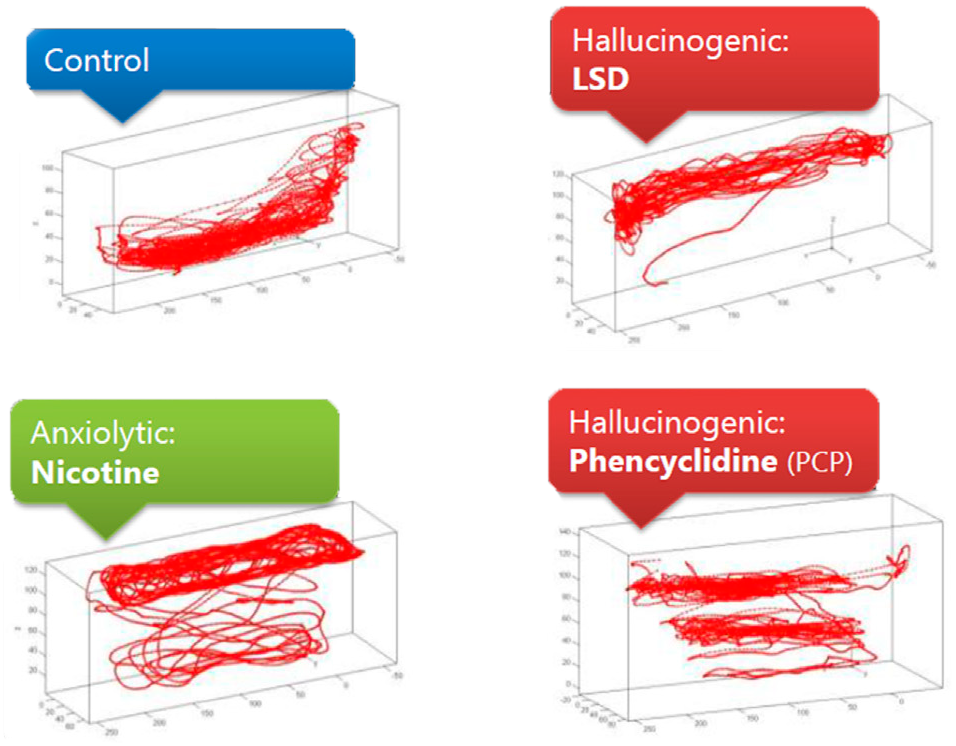
\includegraphics[width=0.8\textwidth]{drug_effect}
	\caption{Zebrafish swimming behaviour under influence of drugs, by \cite{Stewart2015}}
	\label{fig:drug_effect}
\end{figure}



\section{Tracking of Zebrafish}

\begin{itemize}
	\item General setup - aquarium, camera, recordings
	\item Automated or manual annotations - what is trajectories
	\item Tracking requires? - What kinds of detection
	\item More fish, leads to occlusions
	\item Occlusion occurred, now what? - Manual vs automated
	\item Predictions - how is it done?	
\end{itemize}

To investigate the difference in behavioural patterns, i.e. due to drugs, each zebrafish must be detected individually over time. Detection of the zebrafish is often done with automated tracking system, as done by \cite{Stewart2015}, as manual annotation of the data often proves infeasible.

\subsection{Tracking Requirements}
Talk about different viewpoints - side view, top view, advantages and disadvantages.\\
FPS "requirements" - refer to Malte's report?\\
Pre processing?\\

In order to be able to track zebrafish, collection of data is firstly necessary. Recording of the zebrafish is done using one or more cameras either from the top of the aquarium or looking into the aquarium from the side.

Due to the erratic movement of the zebrafish, the higher the \gls{fps} the camera is able to capture video at, the better, as this will increase the probability of the camera capturing every movement of the fish. \cite{Pedersen2017} states, that even at 240 \gls{fps} the zebrafish is still somewhat blurred when accelerating, which can lead to a lower detection rate.

Using the top down view of the aquarium when recording, is often used when using a single camera setup. The top view takes advantage of the uniform and rigid head physiology of the zebrafish. Even though the zebrafish is able to contort it's body, the head most often remains the same, when using the top view. Examples of the rigid head is shown in \autoref{fig:rigid_head}.

\begin{figure}[H]
	\centering
	\begin{subfigure}[b]{0.3\textwidth}
		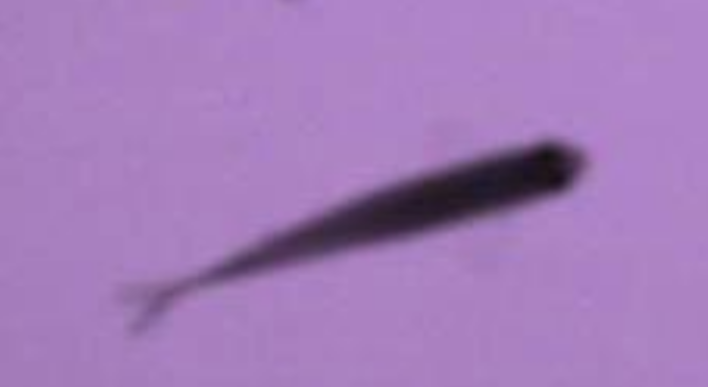
\includegraphics[width=\textwidth]{head_straight}
		\label{fig:head_straight}
	\end{subfigure}
	\begin{subfigure}[b]{0.3\textwidth}
		
\includegraphics[width=\textwidth]{head_bend}
		\label{fig:head_bend}
	\end{subfigure}
	\begin{subfigure}[b]{0.3\textwidth}
		
\includegraphics[width=\textwidth]{head_bend2}
		\label{fig:head_bend2}
	\end{subfigure}
\caption{Examples of the rigid head of the zebrafish in different grades og contortions of the body}
\label{fig:rigid_head}
\end{figure}

The data shown in \autoref{fig:rigid_head}, is captured from above the aquarium with a \gls{nir} backlight beneath the aquarium.\\

When recording from the side of the aquarium more details of the fish is available, as the zebrafish has uniquely coloured stripes on both sides, which can be used to identify the zebrafish \citep{Karpova2018}.

According to \cite{Qian2017}, due to the shape of the zebrafish, it generally takes up more space when filmed from the side than from a top view. Furthermore, when the zebrafish turns towards or away from the camera, the shape will be very different than when looking at the side of the zebrafish \citep{Pedersen2017}. Examples of both a regular side view and some issues from the view is shown in \autoref{fig:side_view}.

\begin{figure}[H]
	\centering
	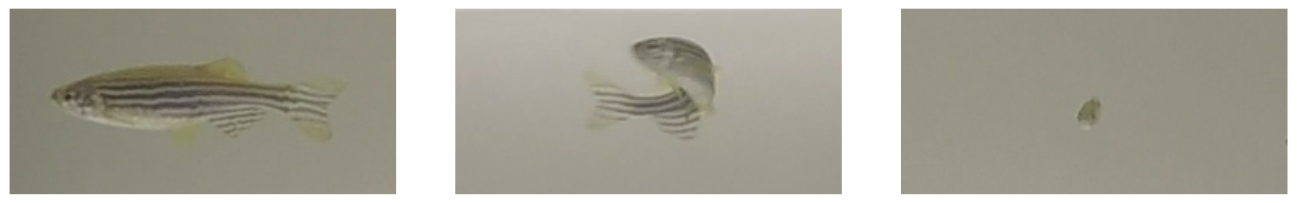
\includegraphics[width=0.9\textwidth]{side_view}
	\caption{Examples of positions of zebrafish in the side view. Image from \cite{Pedersen2017}}
	\label{fig:side_view}
\end{figure}

When data is acquired, it will need to be prepared before tracking or annotation is done. 

\subsection{Annotating Data}
General annotations, but also different "focus points" on the fish. What coordinate is extracted?\\
Kinds of detections.\\

Annotating data using an automated solution can also be defined as a tracking system, whereas annotating data may be understood as manually mark each zebrafish in every frame of the video. 

A tracking system can be split into multiple steps:

\begin{itemize}
	\item Pre processing
	\item Detection
	\item Create trajectories
\end{itemize}

\subsubsection{Pre Processing}
When making operations on a video, the file is split into individual frames, and every frame is treated as an individual image. Before locating of the zebrafish in the image is done, some pre processing of the image is performed. This often includes removing the background and noise from the image.

This is done to ease the process of locating the zebrafish as it will be isolated in the image.

\subsubsection{Detection}
Detection of the zebrafish is done in multiple different ways. A detection will ultimately produce a single point in the image.

Head detection of the zebrafish is often an approach used due to the rigid head of the zebrafish. This means the head will keep the same shape while swimming, whereas the rest of the body may change shape, which will make it harder to detect if focus is on the entire zebrafish.

Other examples of detection, are centre of mass of the zebrafish or extracting a skeleton of the zebrafish, representing the shape of the object with a line. Finding the centre of mass of the zebrafish, if not being limited, may end up outside of the object if it is bending into a shape looking like a C.

Examples of extracted points from detections are shown in \autoref{fig:det_point}.

\begin{figure}[H]
	\centering
	
\includegraphics[width=\textwidth]{det_point}
	\caption{Examples of extracted points from detections}
	\label{fig:det_point}
\end{figure}

\subsubsection{Create Trajectories}
When the desired point in the zebrafish is extracted, the point needs to be linked together to create a trajectory. If only a single zebrafish is present in the aquarium no identification is necessary, as every point found belongs to one individual.

As soon as multiple fish are present in the aquarium at the same time, a decision need to made to connect the previous frame's detections to the new ones in the current frame. This can be done by predicting where each individual will be in the following frame based on a state vector and experience from previous frames as input to a Kalman filter, which then makes a qualified guess based on statistics of the new positions. Besides a Kalman filter, a simple cost function such as the Hungarian algorithm can be applied.\\

An issue occurring when multiple zebrafish are in the same aquarium, is when two or more individuals lie close enough together, or on top of each other, to confuse or trick the predictive and cost algorithm.

\subsection{Occlusions}
According to  \cite{Green2012} the use of automated tracking systems perform with same accuracy as manual annotations but in a faster manner. However, they state that automated tracking systems have complications e.g. occlusions. An occlusion is an overlap of two objects in an automated tracking system, and due to the social behaviour of the zebrafish, occlusions occur often when zebrafish are tracked.

\subsection{Handling Occlusions}
According to a study by \cite{Qian2017}, occlusions will occur both while recording from above and from the side of an aquarium, but with greater occurrence from the side of the aquarium due to the shape of the zebrafish. When an occlusion occurs, the trajectory and unique ID of a zebrafish can be lost and will need re-identification either automatically or manually. If the re-identification is not done correctly, the zebrafish could be given a new or wrong ID which will complicate the tracking data \citep{Feijo2018}. This is shown in \autoref{fig:re-id_Ex}

\begin{figure}[H]
	\centering
	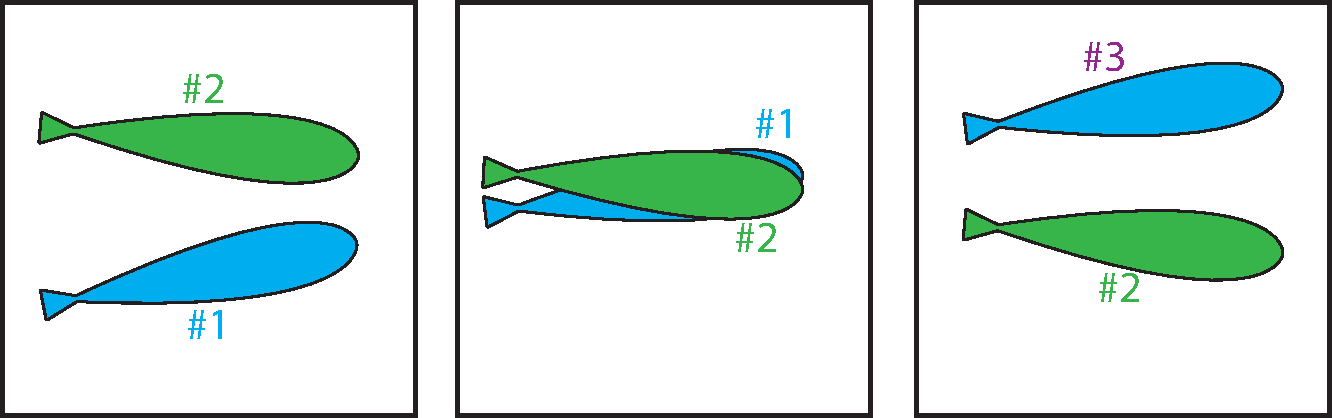
\includegraphics[width=0.9\textwidth]{re_id_ex}
	\caption{Re-ID scenario due to occlusion}
	\label{fig:re-id_Ex}
\end{figure}

Not all occlusions will cause the same types of complications, and some occlusions do not cause any disruption of the trajectory. This is determined by the detection system deployed to track the zebrafish. If the detection of a zebrafish is centred at the head, no occlusion will be detected when the bodies of two zebrafish overlap, however, if detection is done by skeletonisation of the zebrafish, an occlusion will occur (Fig. 2).\\

\begin{figure}[H]
	\centering
	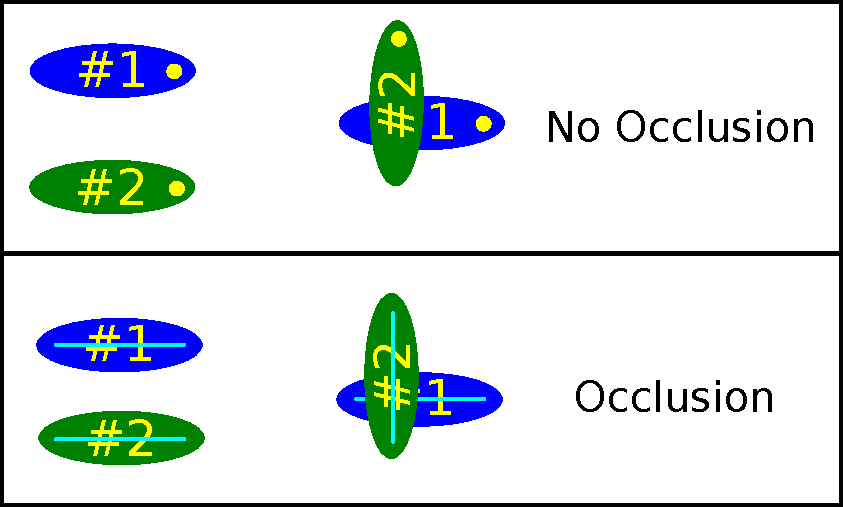
\includegraphics[width=0.85\textwidth]{system_dep_occl}
	\caption{Different types of detection leads to different types of occlusion}
	\label{fig:system_dep_occl}
\end{figure}

A solution to missing tracking data due to occlusions, is to re-link parts of the trajectories (tracklets) to create complete trajectories. This can be done by computing a state vector for each zebrafish and using a Kalman filter which makes predictions of the fish’s position, and thereby estimate what ID belongs to the different zebrafish after an occlusion \citep{Feijo2018, Qian2014}.



To avoid patching in missing data, another more feasible solution could be made to solve occlusions before they occur by detecting the zebrafish in each frame. Both \cite{Romero-Ferrero2019} and \cite{Dolado2014} propose solutions which detect occlusions in an effort to solve them using computer vision. \cite{Dolado2014} has categorised occlusion types by how the zebrafish overlap each other in an effort to specify the solution. However, the only way they solve the occlusions are through a two-step trial and error process i.e. if the first step does not solve the solution, the second step is applied, without factoring in the occlusion type. 
However, a novel approach could be to recognise an occlusion type in order to apply a predefined optimal solution.

\section{Problem Specification}
In order to be able to categorise different occlusions for system, a detection and classification of occlusions is necessary.

To solve this, some preliminary questions are set up:
\begin{itemize}
	\item How do we detect an occlusion in an image?
	\item How can the occlusion be categorised?
	\item Which types of occlusions are the most frequently occurring?
	\item What solution techniques are there? 
	\item What solution techniques Can be applied to each occlusion type?
\end{itemize}
\graphicspath{{figures/research/}}
\chapter{Related Work}\label{ch:related}
As stated in \autoref{ch:intro}, tracking is dine in multiple different ways and so is the handling of occlusions. The different tracking solutions also enables different approaches to handling the occlusions.

The chapter will focus mainly on solutions which aspire to handle the occlusions in some way, as these may yield the most information towards developing a solution in the project.

\section{Detection}
Before doing any kind of tracking of the fish in the aquarium, a detection of every object is necessary to be able to gather the required information for tracking. The detection often relies on a high contrast between the desired objects and the background, making the BLOB extraction more simple \citep{Delcourt2018}. The detection step will be defined as the operations made on each frame in a video producing the coordinate of the fish which is then tracked in the following step.\\

According to \cite{Delcourt2018} the detection methods used by multiple different solutions can be dependent on the resolution of the image. Due to identification solutions relying on colour difference between the objects, high resolution images are necessary to be able to properly differentiate between the objects \citep{idtracker2014, Feijo2018, Romero-Ferrero2019}, as the high resolution often leads to each fish being made up of more pixels than in the low resolution images.

When dealing with lower resolution video \cite{Dolado2015} uses a background subtraction from the original image to remove noise in the image. Afterwards a median filter is used to preserve edges and remove the semi-transparent fins of the fish. Lastly segmentation is done converting the image from greyscale to binary using a threshold. Meanwhile, a filter sorts out \gls{blob}s deemed too small to be fish using a size threshold \citep{Dolado2015}.

Similar to \cite{Dolado2015}, \cite{Rodriguez2017} uses a threshold to segment the fish \gls{blob}s from the background image. A size filter is also applied to remove noise and unwanted false positives. Due to the higher resolution data, more information is added to every detection. A square, denoted as a \gls{roi} is drawn around each \gls{blob} and the area is used to generate further information about the \gls{blob}. The information consists of the centre of mass position, the pixel size of the \gls{blob}, a histogram of the \gls{roi} and the time of detection. The information also includes Hu's Seven Moments Invariants, which are used to characterise patterns in images and can be used to identify rigid and moving objects regardless of orientation in the image \citep{Rodriguez2017}.

\cite{idtracker2014} uses a background subtraction which is calculated from the average image of the whole video used for input. As in the other solutions, a threshold is set to segment the \gls{blob}s from the background. To be able to identify each fish in the image, \cite{idtracker2014} collects a set of images of each individual \gls{blob} in the arena. When operating on the video the reference images collected are used to be able to identify each unique \gls{blob} in the image \citep{idtracker2014}.

\cite{Wang2017} and \cite{Pedersen2017} uses head detection of the fish relying on \gls{doh} in scale space with an \gls{svm} classifier to determine if a detection is a fish head or not. \cite{Pedersen2017} utilises \gls{surf} to extract the features of the fish.

\cite{Qian2014} also utilised scale space \gls{doh} \gls{blob} detection, but instead of using an \gls{svm} classifier, extreme points are found and ellipse fitting is done to locate the head of the fish.

\cite{Romero-Ferrero2019} also utilises background subtraction and applies a size dependent filter to eliminate smaller \gls{blob}s, which are not fish, from the image. Furthermore an intensity threshold is used to distinguish the \gls{blob}s from the background.\\
%Utilising a \gls{cnn}, \cite{Romero-Ferrero2019} is able to detect if two \gls{blob}s are occluding each other.

When detections are made, the tracking is done by connecting the points detected on the fish. This is solved in multiple different ways.

\section{Tracking}
When successful detections are made, the tracking is to link each detection together for each individual \gls{blob}.\\


The low resolution pre processing solution made by \cite{Dolado2015} uses an already commercial tracking solution called \textit{Image-Pro Plus} to track the fish.

A way to connect the desired point on each of the \gls{blob}s is by using the Hungarian algorithm, as done by \cite{Rodriguez2017} and \cite{Pedersen2017}. This is a cost function using the distance between points in two consecutive frames. Both the solutions use the Hungarian algorithm paired with a Kalman filter. The Kalman filter is used to predict the upcoming placement in the following frame, based on previous frames and a state-vector for the fish.

By having identified every fish in the an image, \cite{idtracker2014} are able to track each fish by connecting the centre of mass point of the same identified object in concurrent frame. If a \gls{blob} is recognised as more than one individual, handling of the occlusion is necessary before the tracking can take place.

By using the centre of the fitted ellipse on the fish \cite{Qian2014} uses a state vector consisting of the position and the speed of each individual in $ x $ and $y$ direction. The state vector is used by a Kalman filter to predict the fish's position. To accompany the Kalman filter prediction, \cite{Qian2014} uses feature matching to verify the the predictions made. 

\cite{Wang2017} also uses a Kalman filter prediction paired with a \gls{cnn} based identification to track the fish.

\section{Occlusion Handling}
During tracking, occlusions can occur and in order to have complete trajectories these must be handled. Some solutions chooses not to handle these and have some missing data points, other solutions handles these occlusions in different manners.

\cite{Dolado2015} uses a single image solution to handle occurring occlusions. They have categorised occlusions into two different types, with two different solutions. By defining a size threshold larger than the observed size of one fish, the \gls{blob}s consisting of two fish or more are segmented in the image. The two different categories of occlusions are an elongation of the fish, making one long \gls{blob}. The other category is when the fish either cross or create a T-like shape \citep{Dolado2015}.

The elongation is handled by eroding the image and then dilating to just before the two \gls{blob}s connect to create only one. To handle the crossing, resulting in an X- or T-shape, an ellipse fitting is made around the \gls{blob} and it is then separated by the shortest axis of the ellipse \citep{Dolado2015}.

\cite{Rodriguez2017} does not state how occlusions are handled, other than when identification is not possible, the \gls{blob} is not assigned to an identification.

By detection the heads of the fish, \cite{Qian2014} are able to distinguish two fish from each other even though a crossing of the bodies occur. If two fish are in a close proximity and a head is close to another fitted ellipse, an angle constraint from the ellipse fitting is applied which is able to differentiate the two and detect the head. Should a head of the fish be occluded, the solution will produce an error and not be able to track the occluded fish at that point. Instead a compensation window of the previous state of the fish is used and the new position of the fish is estimated \citep{Qian2014}. 

\cite{Wang2017} handles occlusions depending on the amount of time the individual is occluded. If the fish is occluded for no more than five consecutive frames, an assumption of the continued predicted path is made based on a constant velocity. If the fish is occluded for longer than five frames, the fish is re-identified by the \gls{cnn} and the trajectory will be missing data from the time it is occluded.

\cite{idtracker2014} has two ways of handling occlusions. Firstly an erosion is attempted as a solution which can often lead to separating two \gls{blob}s from each other. If two individuals are still touching or one is occluding the other, the second step is initiated. Using the identification, the fish which are not in the occlusion are identified, to lower the amount of fingerprints to search for in the occlusion. The average velocity of the fish in the occlusion is found, using the speed of the fish necessary to take part in the occlusion,  if this speed exceeds a threshold, the fish is ruled out. If this does not yield a solution to the issue the individuals are left without an identity.

The newer solution of idtracker, idtracker.ai by \cite{Romero-Ferrero2019} uses a \gls{cnn} to detect occlusions. This network is trained using images of both single animals and occlusions. Then by using the second \gls{cnn} used in th solution, used for identification, is used to identify the two animals taking part in the occlusion. by training the identity network on the images from the data which does not contain occlusions, the identity network is able to identify the animal even though occlusions occur \citep{Romero-Ferrero2019}. It is not mentioned how the solution handles an occlusion of which one individual is completely covered by another.

\todo{Skriv en outro for afsnittet, som skal lede ind i en problem analyse.}
\graphicspath{{figures/intro/}}
\chapter{Analysis}\label{ch:analysis}



\section{Behavioural Analysis of Zebrafish}
Zebrafish are very social animals and have tendencies to form groups \citep{RahmanKhan2018}. An aggregation of zebrafish can be either a shoal or a school depending on whether the zebrafish are interacting socially or not. When an aggregation of zebrafish is due to social interaction, the zebrafish are shoaling and the swimming pattern is chaotic, but when zebrafish are schooling, the swimming pattern is tightly coordinated and organised \citep{Miller2012a}. Identification of the swimming pattern can thereby be studied to investigate social phenotypes and behavioural patterns when affected by a certain drug or pheromone \citep{RahmanKhan2018}. 

\cite{Kalueff2013} describes multiple scenarios in which the zebrafish is prone to sudden changes in both speed and direction. Depending on the situation, the zebrafish can move very erratic often reflecting a state of anxiety or fear. Furthermore, sudden bursts can also occur in an attempt to attack another fish, often connected to social dominance \citep{Kalueff2013}.

As mentioned, the zebrafish is also used to test the general behaviour when affected by a drug. This is done by having a control group of zebrafish and recording the normal behaviour in an aquarium and then comparing this behaviour with a drug affected behaviour \citep{Stewart2015}. \autoref{fig:drug_effect} shows an example of swimming patterns of zebrafish under influence of different drugs made by \cite{Stewart2015}. It is clear how the drugs changes the swimming patterns of a zebrafish, which may be transferable to how it will affect humans as well.\\ 

\begin{figure}[h]
	\centering
	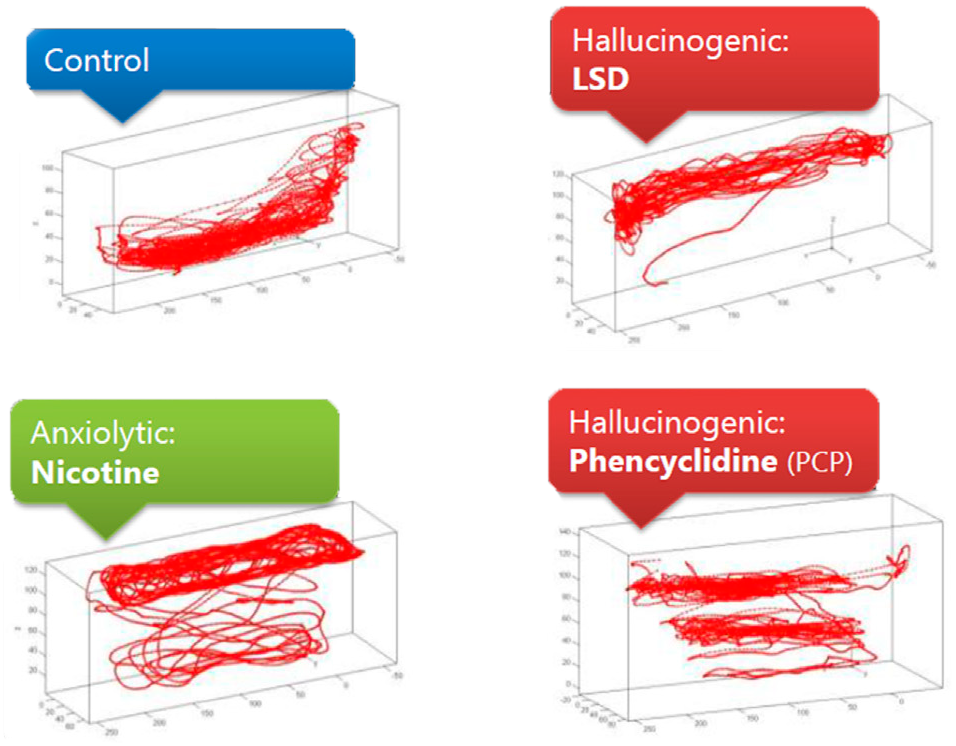
\includegraphics[width=0.8\textwidth]{drug_effect}
	\caption{Zebrafish swimming behaviour under influence of drugs, by \cite{Stewart2015}}
	\label{fig:drug_effect}
\end{figure}


\section{Tracking of Zebrafish}

To investigate the difference in behavioural patterns, i.e. due to drugs, each zebrafish must be detected individually over time. Detection of the zebrafish is often done with an automated tracking system, as done by \cite{Stewart2015}, as manual annotation of the data often proves infeasible.

\subsection{Tracking Requirements}
In order to be able to track zebrafish, collection of data is firstly necessary. Recording of the zebrafish is done using one or more cameras either from the top of the aquarium or looking into the aquarium from the side.

Due to the erratic movement of the zebrafish, the higher the \gls{fps} the camera is able to capture video at, the better, as this will increase the probability of the camera capturing every movement of the fish. \cite{Pedersen2017} states, that even at 240 \gls{fps} the zebrafish is still somewhat blurred when accelerating, which can lead to a lower detection rate.

The top down view of the aquarium when recording, is often used when using a single camera setup. The top view takes advantage of the uniform and rigid head physiology of the zebrafish. Even though the zebrafish is able to contort its body, the head most often remains the same, when using the top view. Examples of the rigid head is shown in \autoref{fig:rigid_head}.

\begin{figure}[H]
	\centering
	\begin{subfigure}[b]{0.3\textwidth}
		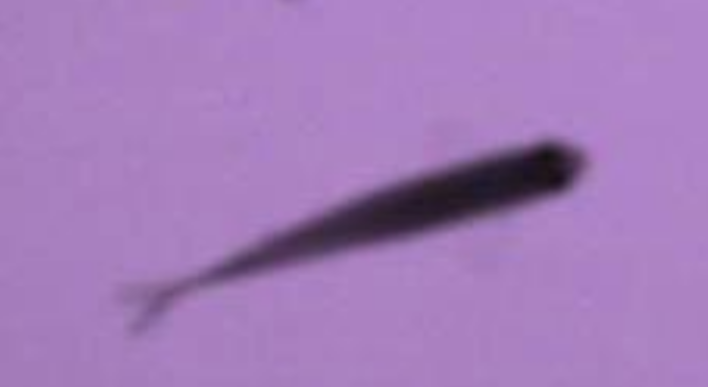
\includegraphics[width=\textwidth]{head_straight}
		\label{fig:head_straight}
	\end{subfigure}
	\begin{subfigure}[b]{0.3\textwidth}
		
\includegraphics[width=\textwidth]{head_bend}
		\label{fig:head_bend}
	\end{subfigure}
	\begin{subfigure}[b]{0.3\textwidth}
		
\includegraphics[width=\textwidth]{head_bend2}
		\label{fig:head_bend2}
	\end{subfigure}
	\caption{Examples of the rigid head of the zebrafish in different grades og contortions of the body}
	\label{fig:rigid_head}
\end{figure}

The data shown in \autoref{fig:rigid_head}, is captured from above the aquarium with a \gls{nir} backlight beneath the aquarium.\\

When recording from the side of the aquarium more details of the fish is available, as the zebrafish has uniquely coloured stripes on both sides, which can be used to identify the zebrafish \citep{Karpova2018}.

According to \cite{Qian2017}, due to the shape of the zebrafish, it generally takes up more space when filmed from the side than from a top view. Furthermore, when the zebrafish turns towards or away from the camera, the shape will be very different than when looking at the side of the zebrafish \citep{Pedersen2017}. Examples of both a regular side view and some issues from the view is shown in \autoref{fig:side_view}.

\begin{figure}[H]
	\centering
	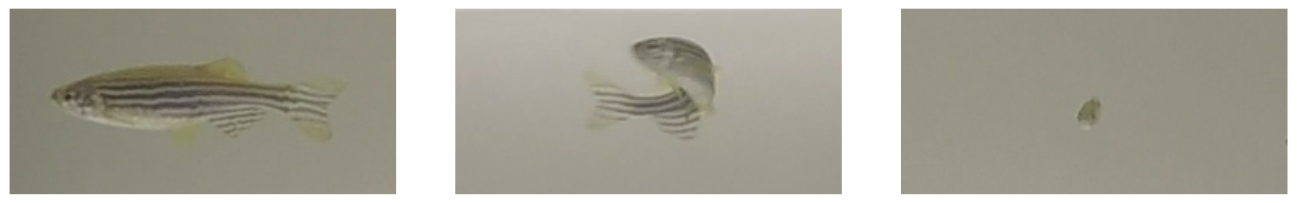
\includegraphics[width=0.9\textwidth]{side_view}
	\caption{Examples of positions of zebrafish in the side view. Image from \cite{Pedersen2017}}
	\label{fig:side_view}
\end{figure}

When data is acquired, it will need to be prepared before tracking or annotating is done. 

\subsection{Annotating Data}

Annotating data is understood as manually marking each zebrafish/object in every frame of a video, whereas, when using an automated solution it can also be referred to as tracking system. 

A tracking system can be split into multiple steps:

\begin{itemize}
	\item Pre processing
	\item Detection
	\item Create trajectories
\end{itemize}

\subsubsection{Pre Processing}
When making operations on a video, the file is split into individual frames, and every frame is treated as an individual image. Before locating of the zebrafish in the image is done, some pre processing of the image is often performed. This often includes removing the background and noise from the image.

This is done to ease the process of locating the zebrafish as it will be isolated in the image.

\subsubsection{Detection}
Detection of the zebrafish is done in multiple ways. A detection will ultimately produce a single point in the image.

Head detection of the zebrafish is an often used approach due to the rigid head of the zebrafish. This means the head will keep the same shape while swimming, whereas the rest of the body may change shape, which will make it harder to detect if focus is on the entire zebrafish.

Other examples of detection, are centre of mass of the zebrafish or extracting a skeleton of the zebrafish, representing the shape of the object with a line. Finding the centre of mass of the zebrafish, if not being limited, may end up outside of the object if it is bending into a shape looking like a C.

Examples of extracted points from detections are shown in \autoref{fig:det_point}.

\begin{figure}[H]
	\centering
	
\includegraphics[width=\textwidth]{det_point}
	\caption{Examples of extracted points from detections. The first fish is head detection, the second is centre of mass, and the third is skeletonisation}
	\label{fig:det_point}
\end{figure}

\subsubsection{Create Trajectories}
When the desired point in the zebrafish is extracted, the point needs to be linked together to create a trajectory. If only a single zebrafish is present in the aquarium no identification is necessary, as every point found belongs to one individual.

As soon as multiple fish are present in the aquarium at the same time, a decision needs to be made to connect the previous frame's detections to the new ones in the current frame. This can be done by predicting where each individual will be in the following frame based on a state vector and experience from previous frames as input to a Kalman filter, which then makes a qualified guess based on statistics of the new positions. Besides a Kalman filter, a simple cost function such as the Hungarian algorithm can be applied to link detections.\\

An issue occurring when multiple zebrafish are in the same aquarium, is when two or more individuals lie close enough together or on top of each other, which may confuse or trick the prediction and cost algorithm.

\subsection{Occlusions}
An occlusion is when one object is hidden or overlapped by another object from a specific point of view e.g. from the camera view. When a zebrafish occlude another there is a risk of losing the detection and thereby the position of the occluded fish in one or more concurrent frames. According to  \cite{Green2012} the use of automated tracking systems perform with same accuracy as manual annotations but in a faster manner. However, they state that automated tracking systems have complications with occlusions. 

When a detection is lost due to an occlusion, the identity of the zebrafish may be lost as well. If no re-identification is employed in a tracking system, a new ID may be assigned to the object which was lost due to an occlusion. This scenario is visualised in \autoref{fig:re-id_Ex}

\begin{figure}[H]
	\centering
	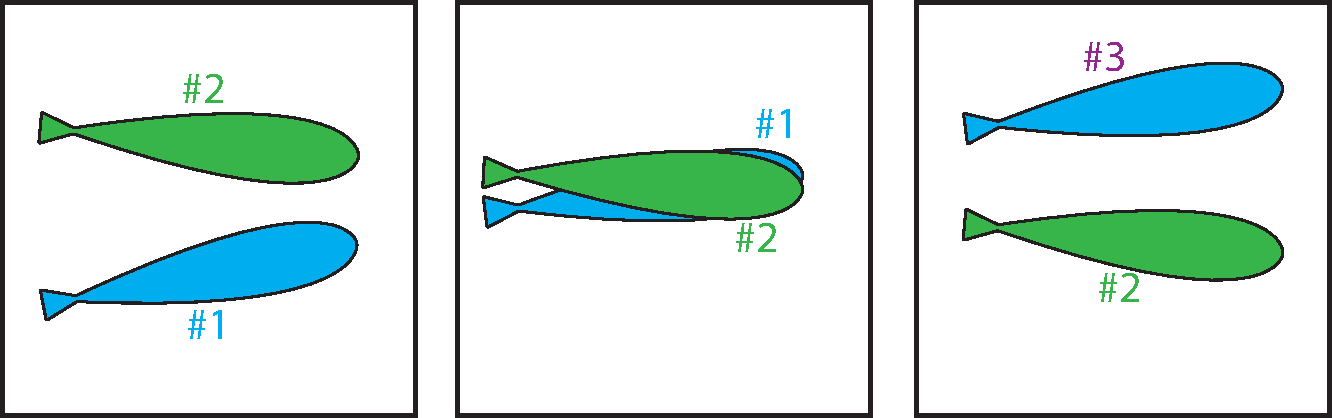
\includegraphics[width=0.9\textwidth]{re_id_ex}
	\caption{Re-ID scenario due to occlusion}
	\label{fig:re-id_Ex}
\end{figure}

Not all occlusions will cause the same types of complications, and some occlusions do not cause any disruption of the trajectory. This is determined by the detection system deployed to track the zebrafish. If the detection of a zebrafish is centred at the head, no occlusion will be detected when only the bodies of two zebrafish overlap, however, if detection is done by either skeletonisation or centre of mass, an occlusion will most likely occur \citep{Feijo2018}. An example of this scenario is shown in \autoref{fig:system_dep_occl}.

\begin{figure}[H]
	\centering
	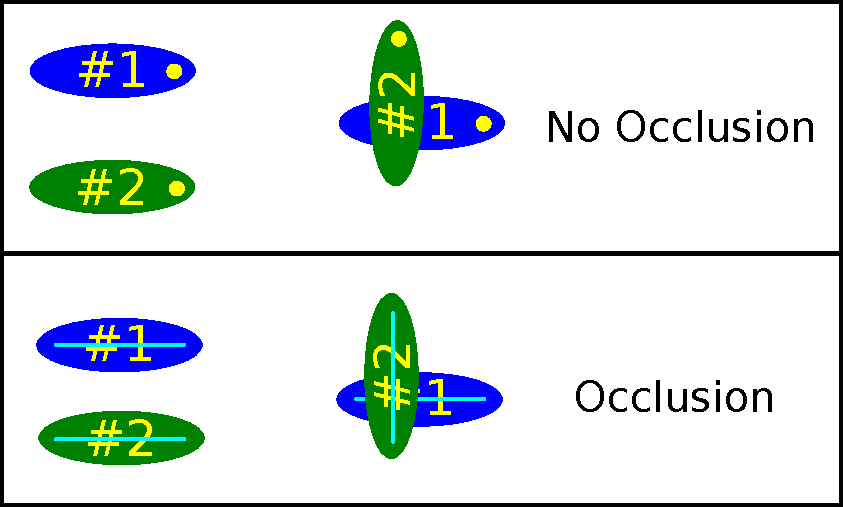
\includegraphics[width=0.85\textwidth]{system_dep_occl}
	\caption{Different types of detection leads to different types of occlusion}
	\label{fig:system_dep_occl}
\end{figure}

Missing detections and wrong identifications are undesirable, as this will require a user of the tracking system to intervene and correct the errors, which will prolong the process. Therefore, solutions to either handling the occlusions or automatically solving the wrong identification are often implemented in a tracking solution.

\subsection{Object Detection}\label{sec:obj_det}
In order to be able to detect the zebrafish occlusions in every frame, object detection is necessary. Object detection is defined as an employment of computer vision which recognises unique features of objects in an image.

Object detection consists of two main tasks; classification and localisation. It can furthermore be split into two categories depending on the amount of classes which must be detected. If it is only one class, such as detecting humans in an image or detecting any kind of zebrafish occlusion, it is known as class-specific detection. Whereas detecting multiple different kinds of objects is knows as multi-class detection  \citep{Zhang2013}.

The main objective of an object detector is to generate a label list of predefined objects detected in an image. The list should specify which classes are present and where in the image they are located.\\

\subsubsection{Deep Learning}
When using deep learning and a \gls{cnn} for object detection one of the earliest implementations was the \gls{rcnn}. As the name suggests, the method is based upon a region proposal based \gls{cnn} instead of using the often previously used sliding window technique which some times can lead to a large amount of testing windows.

The \gls{cnn} used in the \gls{rcnn} is utilised for feature extraction feeding into a class-specific \gls{svm} to categorise each object. The \gls{cnn} is pre-trained on the ImageNet database and then trained on the PASCAL VOC dataset. An overview of the \gls{rcnn} pipeline is shown in \autoref{fig:rcnn_pipe}. More in-depth of deep learning is found in \autoref{ch:design}.

\begin{figure}[h]
	\centering
	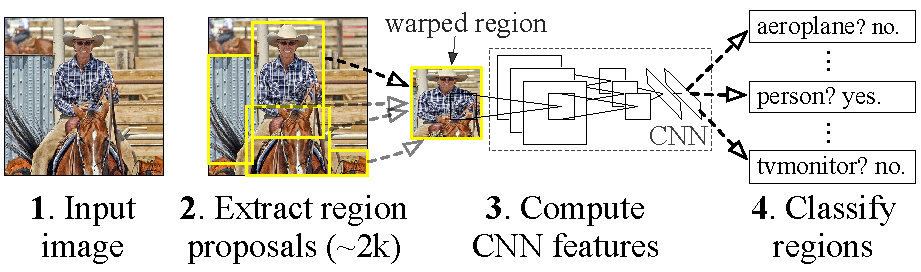
\includegraphics[width=0.9\textwidth]{rcnn_flow}
	\caption{Simple flow diagram of the R-\gls{cnn} by \cite{Girshick2014}}
	\label{fig:rcnn_pipe}
\end{figure}

As shown in \autoref{fig:rcnn_pipe} the \gls{rcnn} is split into 3 individual steps consisting of; region proposals, feature extraction, and \gls{svm} classification.\\

The region proposals are extracted using \textit{SelectiveSearch} which initialises regions in the image and then merge these with a hierarchical grouping \citep{Uijlings2013}. The final grouping is then a box containing the entire image. The regions are grouped in relation to colour space and similarity \citep{Girshick2014}. 

The next step in the solution is warping the proposed regions to fit the \gls{cnn} input size and extracting features from these and produce a $4096$ dimensional feature vector. The feature vectors consist of both positive and negative proposals found with the SelectiveSearch. These vectors are used to train the class specific \gls{svm}s, one \gls{svm} per class in which a background class is included \citep{Girshick2014}.
When testing a given image, the SelectiveSearch generates approximately 2000 proposals, which each are propagated through the \gls{cnn} to extract feature vectors. Each feature vector is tested against every class-specific \gls{svm}. To remove overlapping detections a greedy Non-maximum Suppression is applied \citep{Girshick2014}.

At the time of publication, the \gls{rcnn} achieves state of the art performance in object detection, with a $~13\%$ increase in precision compared to the previously best method \citep{Girshick2014}.

The \gls{rcnn} does leave room for improvements as it is a slow solution when testing on an image. Furthermore, as the solution is split into multiple modules, the loss calculations for training the \gls{svm}s is not used to update the \gls{cnn}.\\

An improvement on both speed and accuracy of the \gls{rcnn} was published a year later, called Fast \gls{rcnn}. Instead of using the multi module pipeline, as illustrated in \autoref{fig:rcnn_pipe}, training is now done end-to-end. The solution takes an image  and a set of pre-computed object proposals, like the \gls{rcnn} \citep{Girshick2015}.

Instead of individual proposals as in the original \gls{rcnn}, the new iteration propagates the entire image forward through multiple convolutional and max-pooling layers to produce a feature map. The features are extracted from each proposal using a \gls{roi} pooling layer. After the \gls{roi} pooling layer follows two fully connected layers leading to two different outputs; a softmax classification layer and a bounding box regression layer \citep{Girshick2015}. This pipeline is also shown in \autoref{fig:frcnn_pipe}.

\begin{figure}[H]
	\centering
	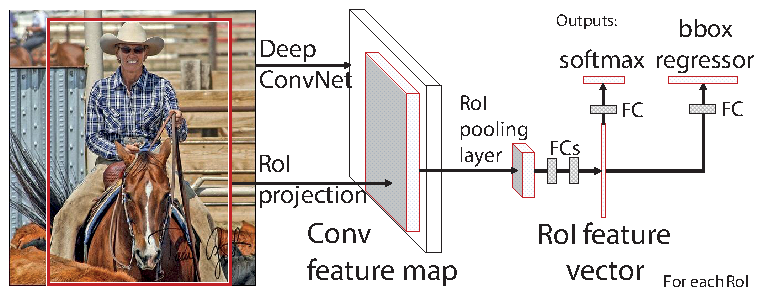
\includegraphics[width=0.9\textwidth]{frcnn_pipe}
	\caption{Fast \gls{rcnn} pipeline overview, by \cite{Girshick2015}}
	\label{fig:frcnn_pipe}
\end{figure}

Just like the \gls{rcnn}, the Fast \gls{rcnn} is pre-trained using the ImageNet database fine tuned for object detection, but instead of being based on AlexNet, as \gls{rcnn} is, the best performing solution of Fast \gls{rcnn} is based on the deeper VGG16 network \citep{Girshick2015}. When comparing to the previous iteration, \gls{rcnn}, it is done while both solutions are using the VGG16 network layout instead of the AlexNet for the \gls{rcnn}. This is done to have a common ground for comparison. Fast \gls{rcnn} improves precision with $4\%$ \citep{Girshick2015}.

The main improvement of the new model is more in speed both in training and testing due to the computing of a convolutional feature map for the entire image. The speed increase is only in relation to the actual detection, as the regions proposals are slow and create a bottleneck for the system \citep{Girshick2015}.\\

To combat the slow region proposals of Fast \gls{rcnn}, \cite{Ren2017} created a third iteration of the \gls{rcnn} network called \textit{Faster \gls{rcnn}}. Here a network named Region Proposal Network (RPN) is implemented to compute region proposals as part of a  network. The RPN shares the convolutional layers and the feature map with the \gls{roi} pooling in the Fast \gls{rcnn}. Due to the layers being computed on the entire image, the time used for proposals generated using the RPN is much lower than of a method such as SelectiveSearch. The RPN, computing region proposals, is the only new part of the Faster \gls{rcnn} compared to Fast \gls{rcnn}.

The results of the Faster \gls{rcnn} in precision are rather small, but the entire computing time of the solution has been significantly minimised, from about $2$ seconds per image to $0.2$ seconds, including region proposals for both timings.

Multiple solutions on the \gls{coco} dataset object detection leader board are still employing the framework of \gls{rcnn} and its predecessors, which shows why the \gls{rcnn} is still a state of the are solution.


\subsection{Handling Occlusions}
According to a study by \cite{Qian2017}, occlusions will occur both while recording from above and from the side of an aquarium, but with greater occurrence from the side of the aquarium due to the shape of the zebrafish. As previously mentioned, occlusions can cause errors, resulting in missing data for an individual due to a new ID \citep{Feijo2018}.\\

A solution to missing tracking data due to occlusions, is to re-link parts of the trajectories (tracklets) to create complete trajectories. This can be done by computing a state vector for each zebrafish and using a Kalman filter which makes predictions of the fish’s position, and thereby estimate what ID belongs to the different zebrafish after an occlusion \citep{Feijo2018, Qian2014}.

To avoid patching in missing data, another more feasible solution could be made to solve occlusions before they occur by detecting the zebrafish in each frame. Both \cite{Romero-Ferrero2019} and \cite{Dolado2014} propose solutions which detect occlusions in an effort to solve them using computer vision. \cite{Dolado2014} has categorised occlusion types by how the zebrafish overlap each other in an effort to specify the solution. However, the only way they solve the occlusions are through a two-step trial and error process i.e. if the first step does not solve the solution, the second step is applied, without factoring in the occlusion type. 
However, a novel approach could be to recognise an occlusion type in order to apply a predefined optimal solution.


\section{System Dependencies}\label{sec:int_dep}
Different types of tracking systems may vary in requirement of user interaction throughout the tracking. The ability of the solution may require the user to interact with the system when occlusions occur in the video data in order to pick the correct path for each zebrafish and thereby solve or fix the data. 

If a solution has a high level of user interaction, localisation of an occlusion may not be a requirement due to the necessary interactions of a user, but recognition of an occlusion occurring in the image may be sufficient.\\

With this analysis a specification of the problem sought out to solve is presented in the following chapter.
%An object tracking solutions consists of multiple steps towards creating complete trajectories for each object in an arena. As stated in \autoref{ch:related}, occlusions often lead to issues in tracking solutions and are often not handled to completion. This leads to missing data which a user must handle either by annotating some of the data themselves or using the data incomplete.
%
%To combat this, some solutions choose to solve the occlusions \citep{Romero-Ferrero2019, Dolado2015}. By being able to detect when an occlusion occurs a process of handling them is initiated.
%
%Both \cite{Romero-Ferrero2019} and \cite{Dolado2015} initially counts the amount of objects in the each frame and compare it to the given amount of object which are supposed to be in the frame.\\
%
%An implementation of an occlusion detection solution can be categorised as a single step in an object tracking system. The detection step would consist of detecting occlusions in every frame, categorising the type of occlusion and extracting the occlusion position in the image. This is also show in an flowchart overview in \autoref{fig:overview_flow}.
%%Problem analyse. Hvad er det jeg/vi vil løse og hvorfor? Skal lægge op til problem formuleringen.
%
%Often, before any kind of detections take place some pre processing of the image is done \citep{Delcourt2018}. This would be any kind of alternations made to the image, which will make it easier to isolate the desired objects from the rest of the image.
%
%An implementation of an occlusion detection solution must be placed before the tracking of the objects in a object tracking pipeline, as the handling of occlusions should be done before extracting positions of each individual in the image. An occlusion detection element of an object detection solution which should be able to distinguish between a single fish \gls{blob} and a \gls{blob} consisting of multiple fish.
%
%If the occlusions are handled before doing any kind of tracking, the tracking solution will face less issues needing a solution to be able to track all objects.
%
%\begin{figure}[H]
%	\centering
%	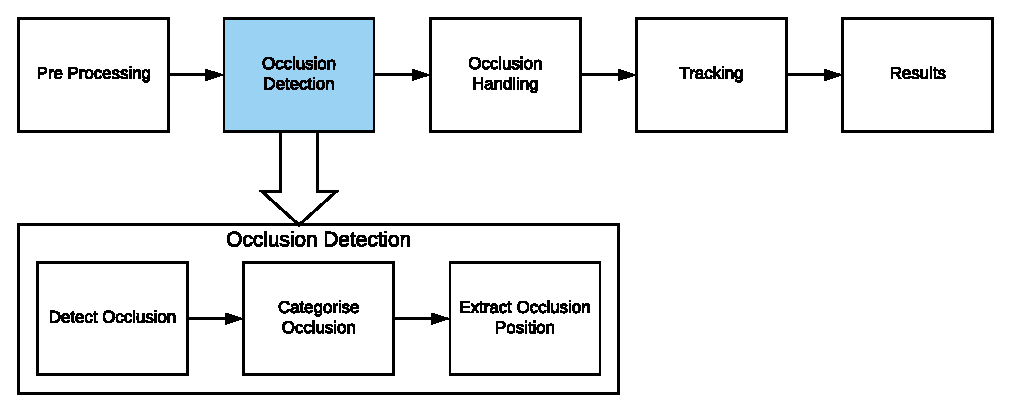
\includegraphics[width=\textwidth]{overview_flowchart}
%	\caption{Overview of an entire tracking system solution and specification of the occlusion detection part.}
%	\label{fig:overview_flow}
%\end{figure}
%
%An occlusion detection solution needs to be able to detect when and where an occlusion is occurring to be able to pass the information on to the occlusion handling process.

\chapter{Problem Statement}
On basis of \autoref{cha:research} \nameref{cha:research} and \autoref{ch:analysis} \nameref{ch:analysis} a problem statement is presented to clarify the objective of this thesis.

\textbf{How can the Loligo Systems object tracker, LoliTrack 4.0, be improved to be able to track objects in deeper water and be prepared for possible 3D tracking?}
\graphicspath{{figures/analysis/}}
\chapter{Data Analysis}\label{ch:data_anal}
%\graphicspath{{figures/research/}}
\chapter{Background Research}\glsresetall
\label{cha:research}
To be able to further develop on the tracking system presented in the \nameref{ch:intro}, background research and system analysis is necessary. In this chapter, the existing Loligo Systems solution LoliTrack is presented as well as the company it self, together with the an overview of tasks to solved for 3D tracking implementation. A further state of the art solutions is presented in \autoref{ch:analysis}.

\section{Loligo Systems}\label{sec:loligo_res}
Loligo Systems is a company who specialise in aquatic biology research, animal physiology, and  behavioural research equipment. The equipment mainly consist of animal chambers, flumes, sensors, instruments and software for automated oxygen consumption measurements, and equipment for video-based tracking and analysis of animal behaviour. Examples of product are shown in \autoref{fig:loliproducts}.

\begin{figure}[H]
	\centering
	\begin{subfigure}{0.33\textwidth}
		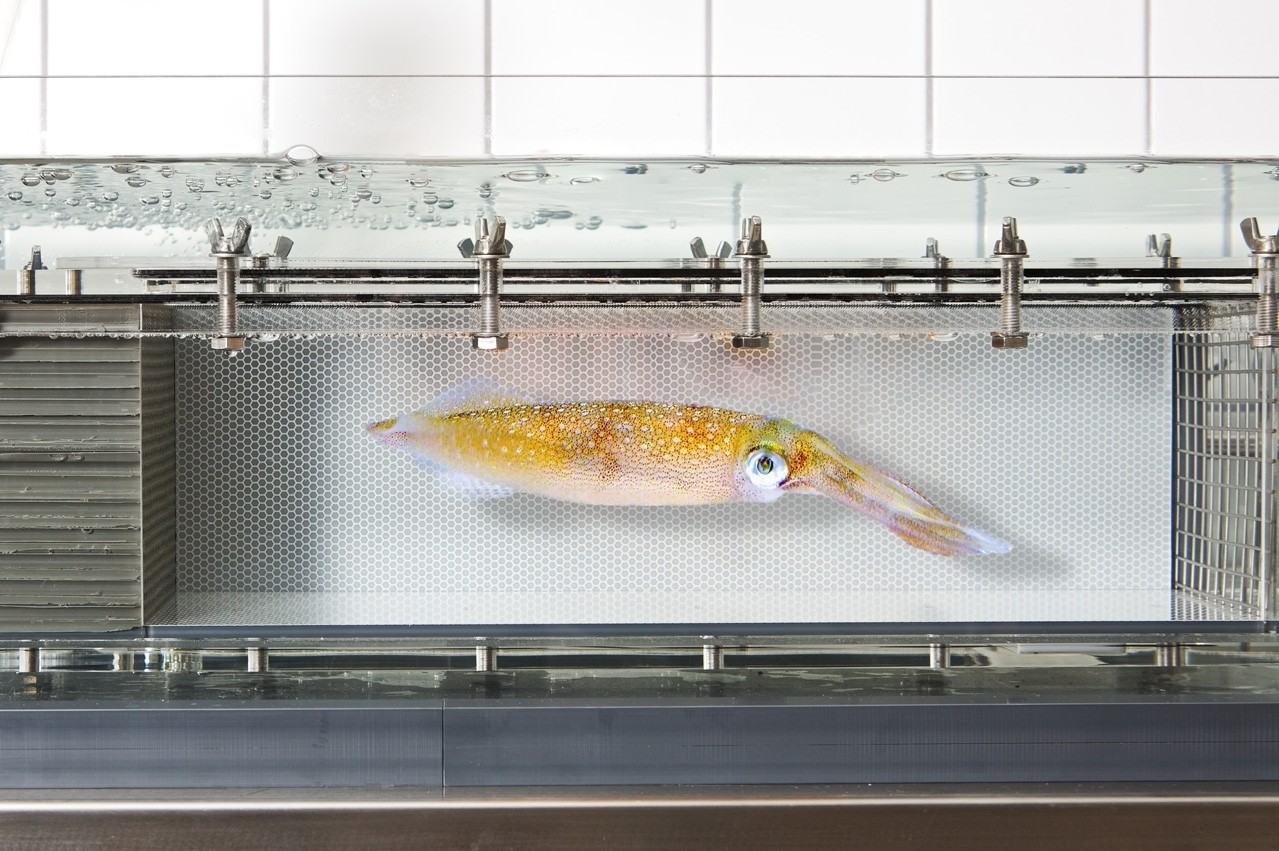
\includegraphics[width=\textwidth]{swimming-performance}
		\caption{Swimming chamber to measure swimming performance.}
	\end{subfigure}
	\begin{subfigure}{0.33\textwidth}
		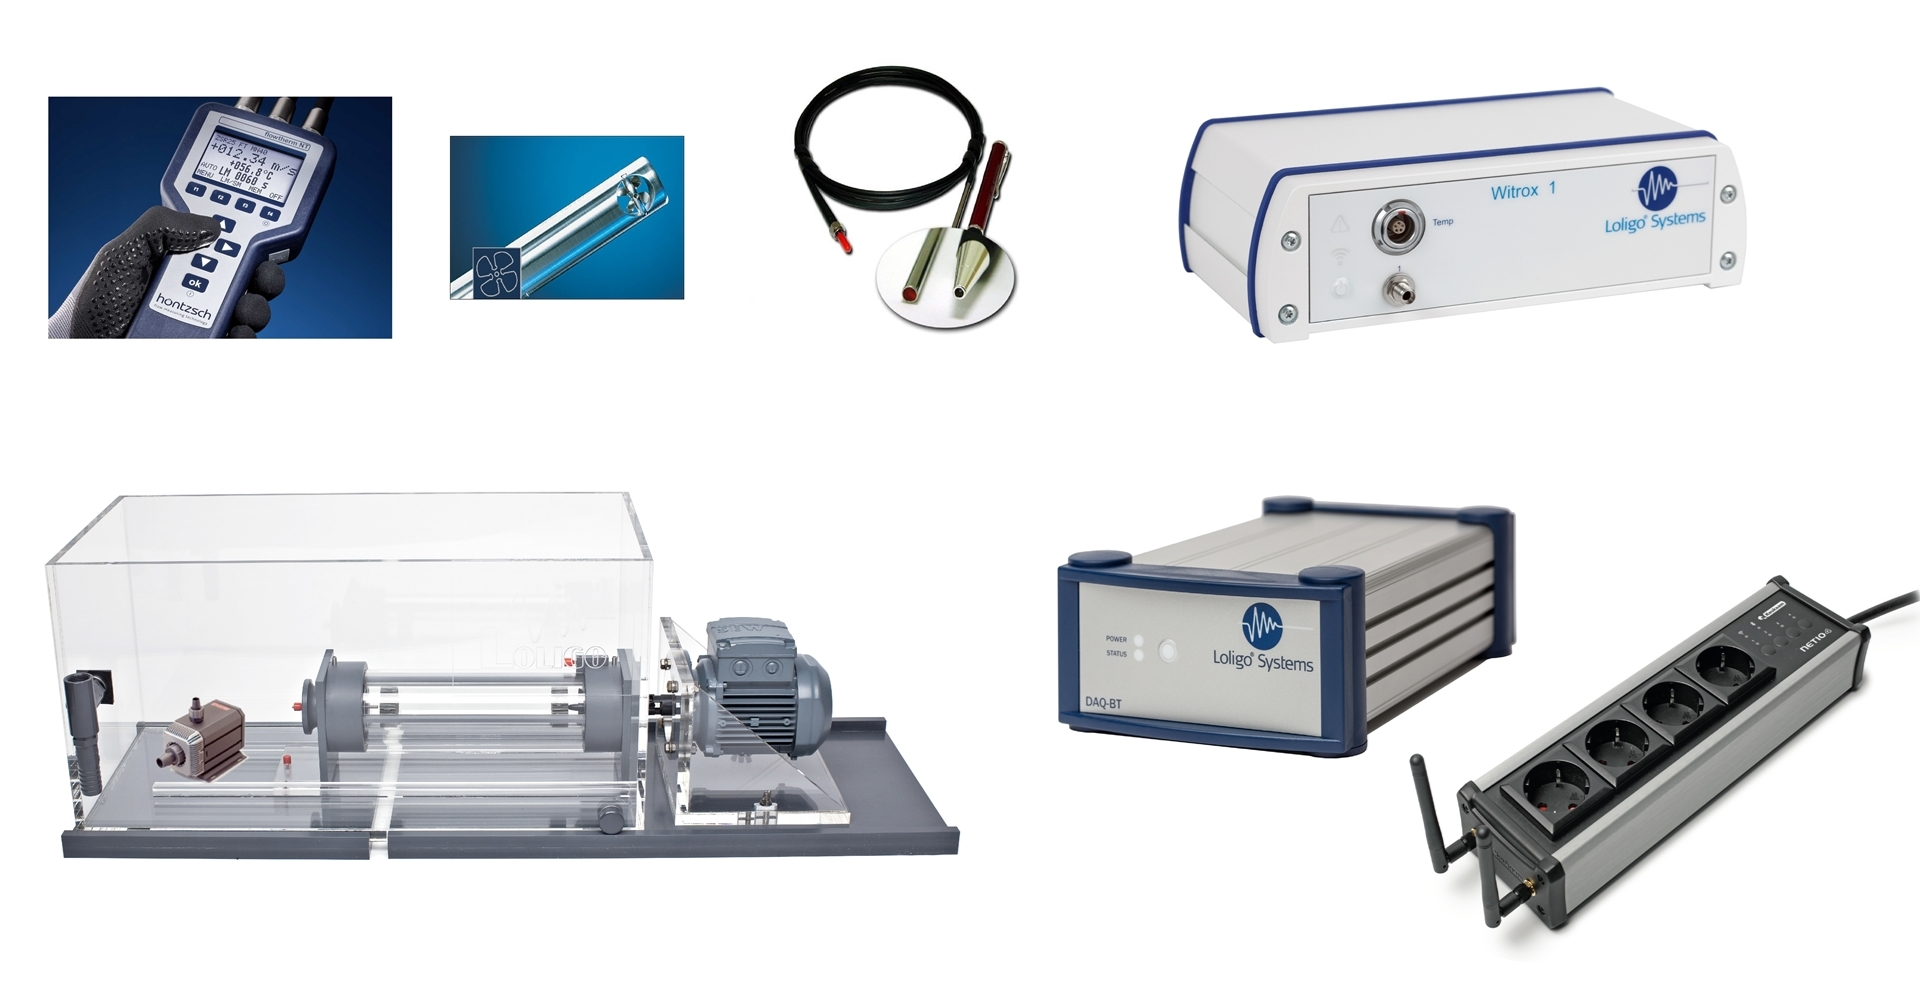
\includegraphics[width=\textwidth]{swimming-respirometry}
		\caption{Swimming chamber fish respirometry. Full package for testing.}
	\end{subfigure}
	\begin{subfigure}{0.32\textwidth}
		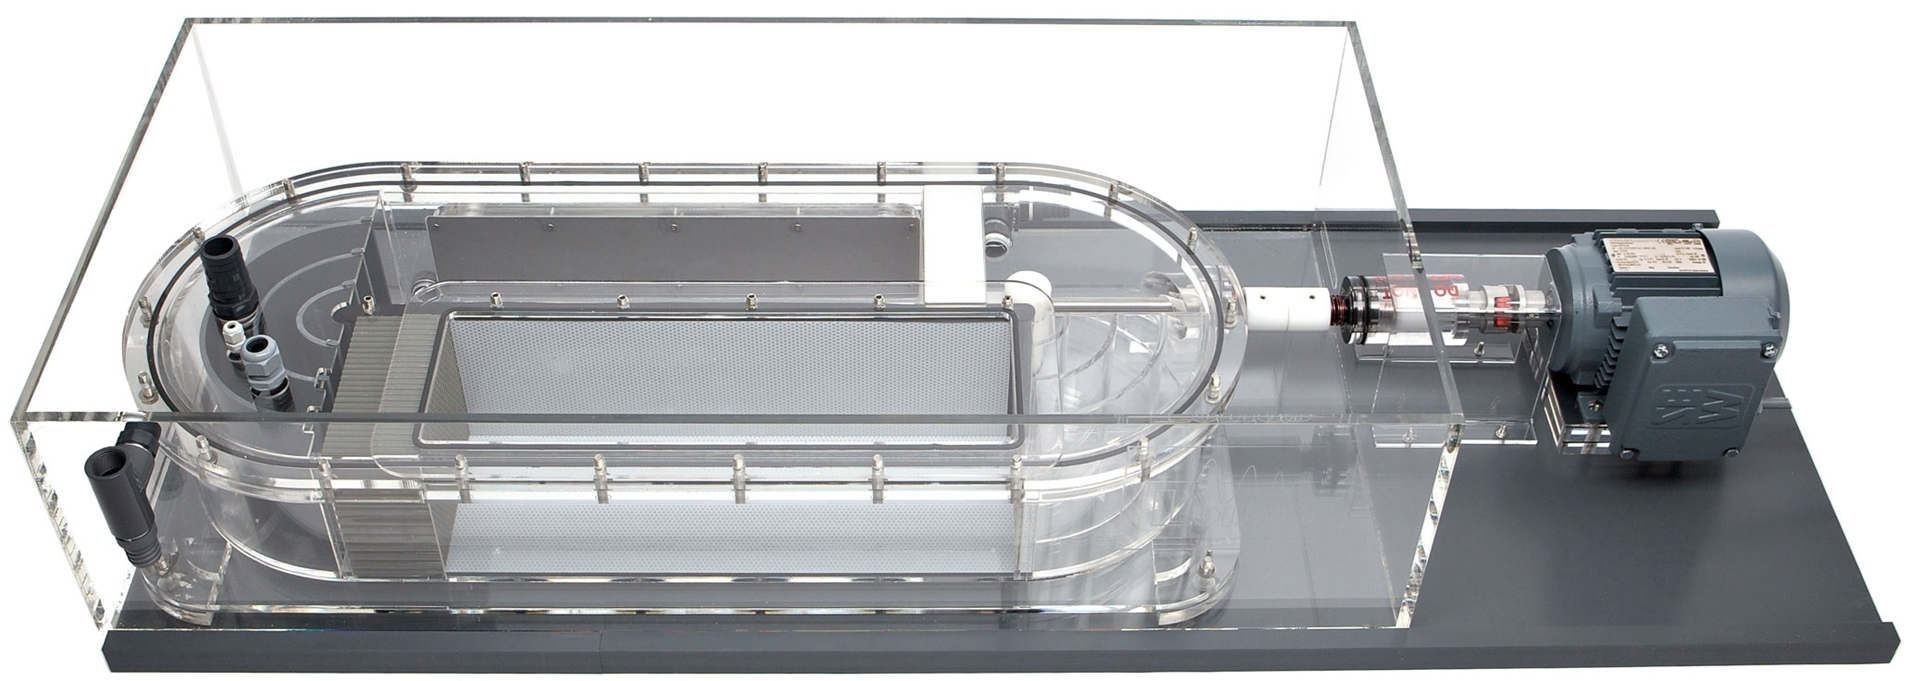
\includegraphics[width=\textwidth]{swim-tunnel-respirometer}
		\caption{Swimming tunnel to test swimming performance under different circumstances.}
	\end{subfigure}
\caption{Overview of a few hardware solution products sold by Loligo Systems}
\label{fig:loliproducts}
\end{figure}

\subsection{LoliTrack}
One of the product developed and sold by Loligo Systems, is the software solution LoliTrack. This is a 2 dimensional tracking solution, which is claimed to be able to track up to 24 objects inside a single arena and able to handle occlusions. The system is made to be used with any camera solution and is contrast based using contrasted background. The software produces an x- and a y-coordinate pair assigned to the centre point of the object tracked. From this data several parameters are produced, consisting of; active/inactive time, velocity, acceleration, direction of movement, direction of orientation, and more. Example images from Loligo's website are shown in \autoref{fig:lolitrack_examples}.

\begin{figure}[H]
	\centering
	\begin{subfigure}{0.45\textwidth}
		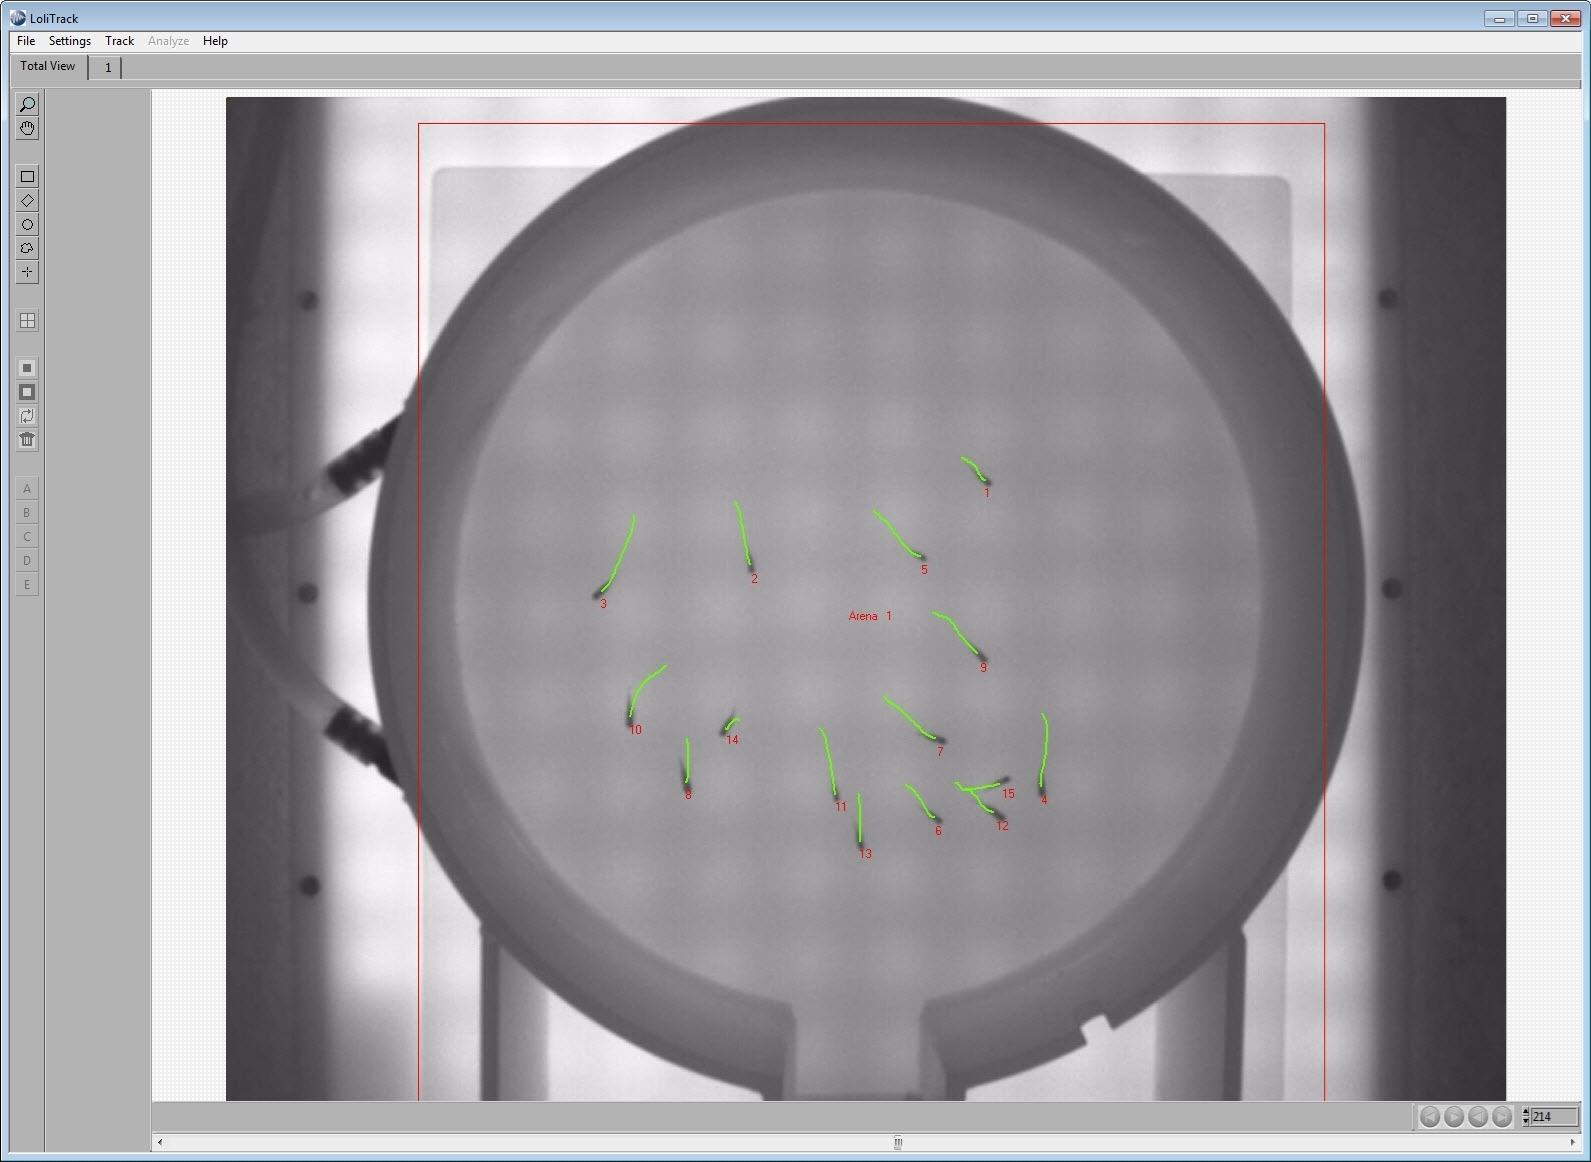
\includegraphics[width=\textwidth]{lolitrack-fish}
		\caption{LoliTrack working on one arena with multiple objects of Zebra Fish}
	\end{subfigure}
	\begin{subfigure}{0.45\textwidth}
		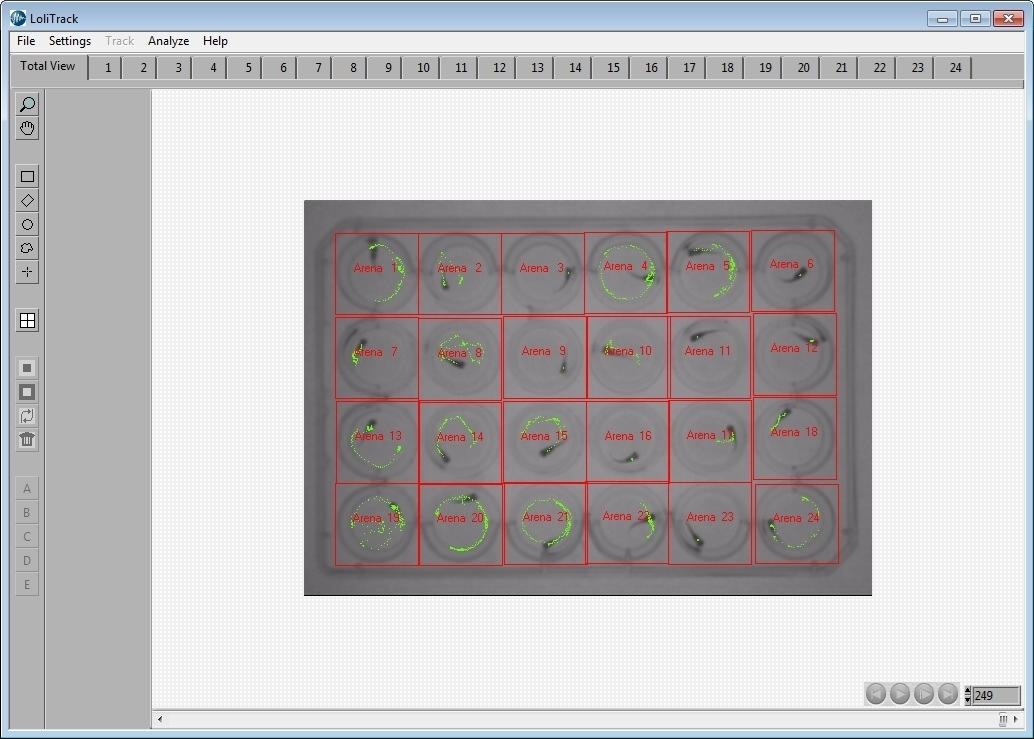
\includegraphics[width=\textwidth]{lolitrack-mult-arena}
		\caption{LoliTrack working on multiple arenas with a single object in each arena}
	\end{subfigure}
	\caption{Overview of a few LoliTrack examples}
	\label{fig:lolitrack_examples}
\end{figure}

According to Loligo Systems the detection and tracking is done in six steps:

\begin{enumerate}
	\item RGB to binary image conversion using the high contrast difference of the fish and background.
	\item Noise reduction using dilation.
	\item Blob identification and extraction.
	\item Pixels in blobs are given a value between $1$ and $3$ dependent on distance to blob centre.
	\item Every blob is fitted with a two-dimensional Gaussian distribution to the values of the pixel values given.
	\item Step 1-4 is repeated for every frame. Afterwards expectations maximisation is used dependent on the previous frames.
\end{enumerate}

\subsection{New LoliTrack Setup}
IDS NIR cameras - NIR backlit aquarium - high contrast between fish an background - undetectable water

\section{Fish Detection}
In computer vision multiple approaches to detect an object exist. The suitable approach depends on the application area and is done both using regular machine learning but also deep learning.

In every scenario, a detection application is an image processing task aimed at detecting the desired objects in an image while refraining from creating false positives. The output should the be at least x-, y-coordinates and a frame number for every detection.

Existing solutions of detection are presented in \autoref{ch:analysis}.

\section{Fish Tracking}
When tracking in two dimensional space, a simple solution is generating tracks by associating the detections made in each frame and minimising the travel distance of the fish in the successive frames.

With multiple fish in the scene, each fish needs to be tracked separately. Having multiple fish can result in occlusions and missed detections, which can lead to faulty tracking because of swapped ID between fish or missing tracks for a period.

Suggested state of the art solutions to tracking fish are presented in \autoref{ch:analysis}.

%\chapter{Project Specification}\label{ch:projecspec}\glsresetall
This chapter specifies the scope of the project. It outlines and delimits the goals for the work conducted, as well as setting the requirements for the solutions implemented during the project work. 

\graphicspath{{figures/design/}}
\chapter{Design}\label{ch:design}
Based on the acquired knowledge from \autoref{ch:analysis} and \autoref{ch:data_anal}, a design of occlusion detection solutions are made. This is implemented using Python3 with the Keras API working with Tensorflow.

This chapter gives an in-depth description of how the implementations are made and the theory behind them.\\

As stated in \autoref{ch:analysis} the use of \gls{cnn}s in object detection is the highest performing solution in different benchmarks. Due to this it is chosen to utilise \gls{cnn}s to perform the occlusion detection of zebrafish. In the following, a description of \gls{cnn}s in general and of the implementation for occlusion detection is presented.

\section{Convolutional Neural Networks (CNN)}
As regular neural networks, \gls{cnn}s are made up of neurons which have learnable weights and biases. Each neuron in the network receives inputs, performs an operation on the input and passes the output on, either linearly or non-linearly, dependent on the design.\\

A \gls{cnn} receives an input image and then transforms this through a series of hidden layers in the network. Each hidden layer consist of a set of neurons, and each neuron is fully connected to the neurons in the previous layer, but does not share any connections inside the layer. The last layer, the output layer, is a fully connected layer and represents the class scores. A \gls{cnn} has neurons arranged in three dimensions, namely: width, height, and depth. Already in the input an RGB image will have a depth of three due to the three colour channels \citep{Karpathy2016b}. A small example of the \gls{cnn} architecture is shown in \autoref{fig:cnn_arch}.

\begin{figure}[H]
	\centering
	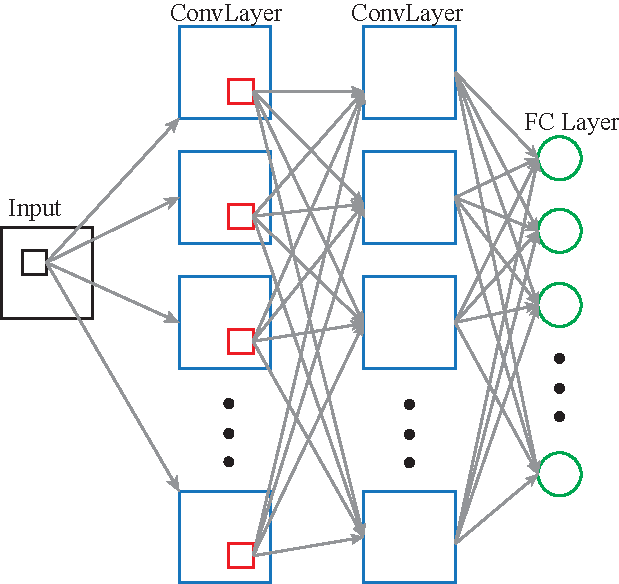
\includegraphics[width=0.6\textwidth]{cnn_arch}
	\caption{Example of a \gls{cnn} architecture}
	\label{fig:cnn_arch}
\end{figure}

\subsection{Layers}
A simple \gls{cnn} will often consist of a sequence of layers, in which each layer transforms one volume of activations to another through differentiable functions. The main layers used are; convolutional layer, pooling layer, and fully connected layer. These layers are presented in the following.

\subsubsection{Convolutional Layers}
The convolutional layer is the main layer of operations in a \gls{cnn}, hence the name of the network type.\\

A convolutional layer operates using a filter also known as a kernel to compute an output by iterating through the input image. This filter convolutes the input using the kernel weights to calculate a dot product of the input. Each filter produces a 2-dimensional activation map. If multiple filters are applied, the 2D activation maps will be stacked along the depth dimension in the output .

Besides being able to control the width and height of the kernel, most often a square, it is also possible to control the depth. Depth is a hyper parameter and corresponds to the amount of filters applied to the input. The neurons along the depth dimension may activate on different edges or colours, but are still focusing on the same region as the rest of the depth column.

When sliding a kernel over an input, a stride can be selected. With a stride of $1$ the filter moves only one pixel at a time, while with a stride of $2$ or higher the filter will move multiple pixels before performing a convolution again.

To enable a kernel to compute all pixels of an input, zero padding is necessary. The size of the zero padding is another hyper parameter, and it allows for controlling the size of the output, mostly for keeping the input size, in height and width, in the output \citep{Karpathy2016b}. A one dimensional example of the influences the different hyper parameters has is shown in \autoref{fig:hyper_ex}.

\begin{figure}[H]
	\centering
	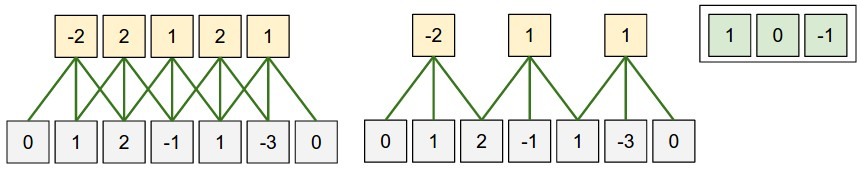
\includegraphics[width=\textwidth]{hyper_ex}
	\caption{With a kernel of [1, 0, -1] the left example shows an input in the bottom with zero padding of size 1 and stride of 1. The right convolution has changed to stride 2 \citep{Karpathy2016b}}
	\label{fig:hyper_ex}
\end{figure}

\autoref{fig:hyper_ex} shows that with a stride of one and employing zero padding, it is possible to keep the dimensions of the input in the output.

The output of a kernel can be calculated using the \autoref{eq:kernel_out}:

\begin{equation}\label{eq:kernel_out}
	(W-F+2P)/S+1
\end{equation}
Where $ W $ is the input volume size, $F$ is the kernel size, $P$ is the amount of zero padding used on the border of the input and, $S$ is the stride. Using the example in \autoref{fig:hyper_ex}, the output can be calculated: 
\begin{equation}
(5-3+2\cdot1)/1+1=5
\end{equation}

The application of stride has some limitations, as the result of \autoref{eq:kernel_out} has to be an integer \citep{Karpathy2016b}.\\

\subsubsection{Pooling Layers}
To be able to control overfitting and to reduce the amount of parameters thereby the computations in a network, pooling layers are often periodically placed in-between successive convolutional layers. A pooling layer reduces the spatial size of the input.

The size reduction is done using a filter in the same way as with a convolutional filter, but no convolutions are performed, instead, dependent on the kind of pooling, a value inside the filter is chosen to be passed on to the ooutput map. Using the most common type of pooling, Maxpooling, often with a filter size of $2\times2$ and a stride of 2, the highest pixel value within the filter is chosen as the output \citep{Karpathy2016b}. An example of this is shown in \autoref{fig:maxpool}.

\begin{figure}[H]
	\centering
	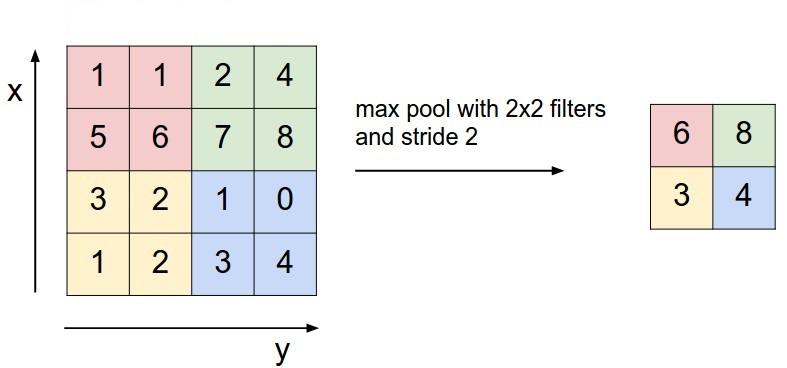
\includegraphics[width=0.8\textwidth]{maxpooling}
	\caption{Maxpooling example with a $2\times2$ kernel and stride 2 \citep{Karpathy2016b}}
	\label{fig:maxpool}
\end{figure}

\subsubsection{Classification}
To be able to use the features extracted from input image in the convolutional layers one or more \gls{fc} layers are added in the end of a \gls{cnn}. As the name suggests, all the neurons in the previous layer are connected to the \gls{fc} layer.

To classify $N$ number of classes, the last \gls{fc} layer has the same amount of neurons as the amount of classes. The output of the last \gls{fc} layer is then the probability of the input image belonging to each class, with a sum of all output neurons being $1$ \citep{Karpathy2016b}.


%\section{Faster R-CNN}
%To be able to detect objects in a frame using a \gls{cnn} the Faster R-\gls{cnn} proposed by \cite{Ren2017} is used. The chosen solution model is the third iteration of the Region based Convolutional Neural Network by \cite{Girshick2014}. As the title proposes, the network is a region proposal based network, used for object detection in an image.

%\subsection{Object Detection}
%Object detection opposed to image classification aims to locate defined objects or instances in images, and often in images containing several objects to locate at the same time, whereas an image classification solution aims to classify one object in an image and recognise the the single object without any localisation.
%
%\subsection{Region-based Convolutional Neural Network (R-CNN)} 
%The model for the R-\gls{cnn} begins with a region search and then do the classification. This model uses \textit{Selective Search} which initialises regions in the image and then merge these with a hierarchical grouping. The final grouping is then a box containing the entire image. The regions are grouped in relation to colour space and similarity \citep{Girshick2014}.
%
%The regions proposed are then fed into the \gls{cnn} which in this case extracts a $4096$ dimensional feature vector. From this feature vector a classification is done using an \gls{svm} for each class \citep{Girshick2014}. \autoref{fig:rcnn_flow} shows the steps in the R-\gls{cnn}.
%
%%\begin{figure}[H]
%%	\centering
%%	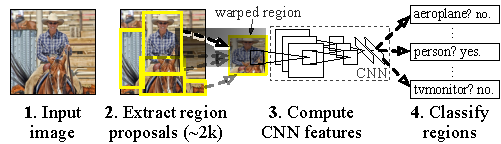
\includegraphics[width=0.8\textwidth]{rcnn_flow}
%%	\caption{Simple flow diagram of the R-\gls{cnn} by \cite{Girshick2014}}
%%	\label{fig:rcnn_flow}
%%\end{figure}
%
%The solution pre-trained on the ImageNet 2012 dataset and is fine tuned using an \gls{iou} greater than $0.5$ with the ground-truth boxes. At the time of development, \cite{Girshick2014} achieves a $62.4\%$ \gls{map} on the Pascal VOC 2012 dataset and $31.4\%$ \gls{map} on the ImageNet 2013 dataset, achieving top position on the leader boards for both datasets.
%
%\subsection{Fast Region-based Convolutional Network (Fast R-CNN)}
%The next iteration of the model by \cite{Girshick2015} is made to reduce time consumption due to the amount of models used to analyse all the regions proposed in the R-\gls{cnn}.
%
%Instead of using the selective search on the entire image, a \gls{cnn} is used to extract features from the image, and the selective search is utilised to detect \gls{roi}s from the feature maps produced by the \gls{cnn} \citep{Girshick2015}.
%
%\subsection{Faster Region-based Convolutional Network (Faster R-CNN)}
%The third iteration of R-\gls{cnn} replaces the selective search with a \textit{Region Proposal Network (\gls{rpn})}, which is a network that generates regions proposals, predict bounding boxes and detects objects.
%
%Here, once again, a \gls{cnn} is used to produce feature maps from the entire image and then uses the \gls{rpn} to propose regions and feed these to a classifier.
%
%The Faster R-\gls{cnn} outperforms the previous iterations in both accuracy and speed. Due to this, the Faster R-\gls{cnn} solution is chosen to utilise for an occlusion detection model.
\section{Image Classification}
A simple occlusion detection can be made without any localisation in order to notify a system of an occlusion present in an image. This is done using an image classification network, trained on two classes; \textit{occlusion} or \textit{no occlusion}.

The network chosen is the VGG16 network, as this is also what the \gls{rcnn} classification network is based upon. An overview of the layers in the VGG16 network is shown in \autoref{fig:vgg16}.

\begin{figure}[H]
	\centering
	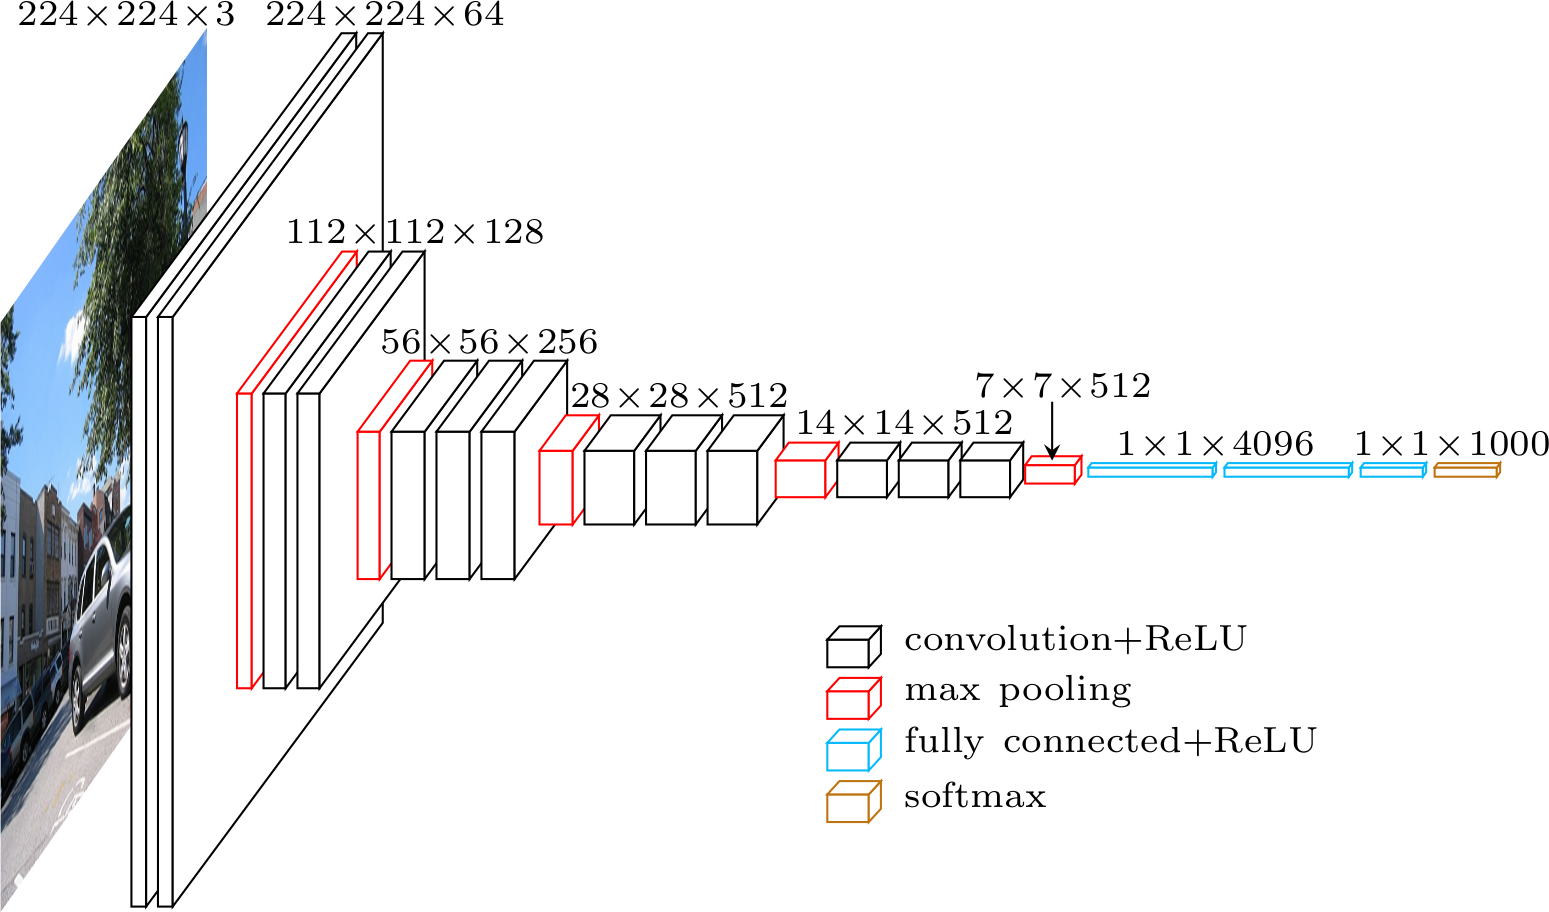
\includegraphics[width=\textwidth]{vgg}
	\caption{VGG16 structure}
	\label{fig:vgg16}
\end{figure}

The network is trained with the pre-trained weights from the ImageNet database. The network can be split into five blocks of convolutions with a max pooling layer after each block.

The images fed into the network are of size $224 \times 224$ and the last fully connected layer has a depth of $2$ due to the amount of classes. The structure of the network is shown in \autoref{tab:vgg16}. \autoref{tab:vgg16} also shows an extra dense layer has been added, and the depth of the \gls{fc} layers has been made smaller.

\begin{table}[H]
	\centering
	\caption{Detailed description of VGG16 design. The input is $224 \times 224 \times3$ images}
	\label{tab:vgg16}
 	\begin{tabular}{lrrrr}
		\textbf{Layer Type}     & \textbf{Feature Map Size} & \textbf{Kernel/Pool Size} & \textbf{Activation}  \\ \hline
		\textbf{Block 1}        &                           &                           &                                     \\
		\rowcolor{lightGrey}  
		Conv2D                  & $64$                      & $3\times3$                & ReLU                                \\
		Conv2D                  & $64$                      & $3\times3$                & ReLU                                \\
		\rowcolor{lightGrey} 
		MaxPooling2D            &                           & $2\times2$                &                                     \\
		\textbf{Block 2}        &                           &                           &                                     \\
		\rowcolor{lightGrey}  
		Conv2D                  & $128$                     & $3\times3$                & ReLU                                \\
		Conv2D                  & $128$                     & $3\times3$                & ReLU                                \\
		\rowcolor{lightGrey}  
		MaxPooling2D            &                       &    $2\times2$             & ReLU                                \\
		\textbf{Block 3}        &                           &                           &                                    \\
		\rowcolor{lightGrey}  
		Conv2D                  & $256$                     & $3\times3$                & ReLU                                \\
		Conv2D                  & $256$                     & $3\times3$                & ReLU                                \\
		\rowcolor[HTML]{EFEFEF} 
		Conv2D                  & $256$                     & $3\times3$                & ReLU                                \\
		MaxPooling2D            &               &          $2\times2$                  &                                     \\
		\textbf{Block 4}        &                           &                           &                                     \\
		\rowcolor{lightGrey}  
		Conv2D                  & $512$                     & $3\times3$                & ReLU                                \\
		Conv2D                  & $512$                     & $3\times3$                & ReLU                                \\
		\rowcolor{lightGrey}  
		Conv2D                  & $512$                     & $3\times3$                & ReLU                                \\
		MaxPooling2D            &             &          $2\times2$                  &                                     \\
		\textbf{Block 5}        &                           &                           &                                    \\
		\rowcolor{lightGrey}  
		Conv2D                  & $512$                     & $3\times3$                & ReLU                                \\
		Conv2D                  & $512$                     & $3\times3$                & ReLU                                \\
		\rowcolor{lightGrey}  
		Conv2D                  & $512$                     & $3\times3$                & ReLU                                \\
		MaxPooling2D            &               &        $2\times2$        & ReLU                                \\
		\textbf{Classification} &                           &                           &                                     \\
		\rowcolor{lightGrey}  
		Flatten                 &                           &                           &                                     \\
		Dense                   & $1024$                    &                           & ReLU                                \\
		\rowcolor{lightGrey}  
		Dense               	& $1024$                    &                           & ReLU                 	           \\
		Dense                   & $512$                    	&                           & ReLU                                \\
		\rowcolor{lightGrey} 
		Dense                   & Amount of Classes         &                           & Softmax                            
	\end{tabular}
\end{table}

\section{Faster \gls{rcnn} Object Detection}
To be able to localise the occlusions in the image and mark them with bounding boxes, an object detection solution is necessary. For this the Faster \gls{rcnn} presented in \autoref{ch:analysis} is implemented. In the following the different objects in the pipeline are described in more detail. An example overview of the pipeline is shown in \autoref{fig:faster_rcnn}.

\begin{figure}[H]
	\centering
	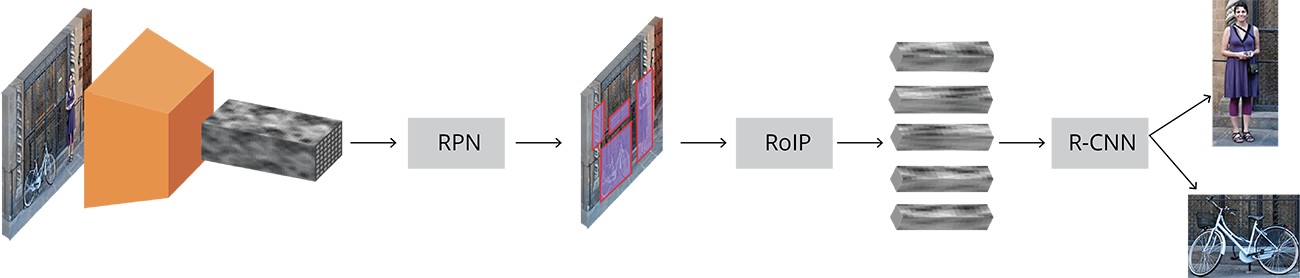
\includegraphics[width=0.9\textwidth]{fasterrcnn-architecture}
	\caption{Overview of the Faster \gls{rcnn} pipeline and its steps \citep{Rey2018}}
	\label{fig:faster_rcnn}
\end{figure}


\subsection{Region Proposal Network}
As mentioned in \autoref{sec:obj_det} \nameref{sec:obj_det}, the Faster \gls{rcnn} utilises a network called \textit{\gls{rpn}} to produce region proposals. The \gls{rpn} shares some convolutional layers with the \gls{cnn}. By sliding a small network over the feature map produced by the last shared convolutional layer \citep{Ren2017}.

As the objective of the object detection is to find bounding boxes in the image, anchors are used. Anchors are fixed bounding boxes of different sizes and ratios and are placed throughout the image. They are used for reference when predicting object locations. An anchor is created for each point in the produced feature map, but the final anchors still reference the input image of the network. The \gls{rpn} outputs a set of good proposals based on the anchors, by having two outputs for each. The first output is an object probability score, the second is bounding box regression for adjusting the anchors to fit potential objects. An example of how anchors are placed in an input image is shown in \autoref{fig:anchors}.

\begin{figure}[H]
	\centering
	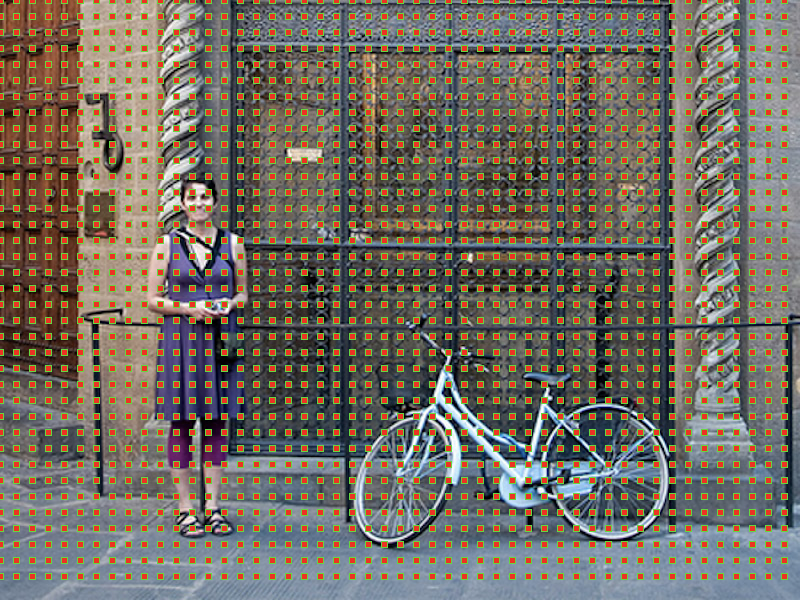
\includegraphics[width=0.6\textwidth]{anchors-centers}
	\caption{Example of anchor centres placed in an input image \citep{Rey2018}}
	\label{fig:anchors}
\end{figure}

For training the \gls{rpn}, the anchors are split into two different categories; the first are those which overlap a ground-truth object with an \gls{iou} of more than $0.7$ which are considered foreground or an object. The second category are those that do not overlap a ground-truth object or have less than $0.3$ \gls{iou}, and are considered background. 
A batch of the anchors is sampled, maintaining a balance between foreground and background anchors. This batch is used to calculate the classification loss using binary cross entropy, and the foreground anchors, only, of the batch to calculate regression loss \citep{Ren2017}.\\

In post processing, \gls{nms} is applied to solve duplicate proposals of one object by discarding the proposals with an \gls{iou} above a set threshold with another proposal with a higher score. A too high \gls{iou} threshold may lead to too many proposals, and too low can lead to missing proposals \citep{Ren2017}.

\subsection{Region of Interest Pooling}
With the object proposals from the \gls{rpn}, the next step is to classify the bounding boxes. But before the classification is done, \gls{roi} pooling is performed. This is done by extracting the fixed size feature maps for each proposal from the already existing convolutional feature map shared \citep{Ren2017}.

\subsection{Classification}
In the classification step of the network the \gls{rcnn} network is employed. With a \gls{fc} layer as output the \gls{rcnn} has two goals; classifying the proposals into classes and to fit the bounding boxes. It flattens the feature map of each proposal and then uses two \gls{fc} layers of size $4096$ with \gls{relu} activation. Then, using two different \gls{fc} layers for each of the objects, one for classification and one for bounding box regression prediction \citep{Ren2017}. An example of the flow of a classification by the \gls{rcnn} is also shown in \autoref{fig:rcnn_ex}. Here a bicycle is classified and the bounding box is adjusted to fit the object.

\begin{figure}[H]
	\centering
	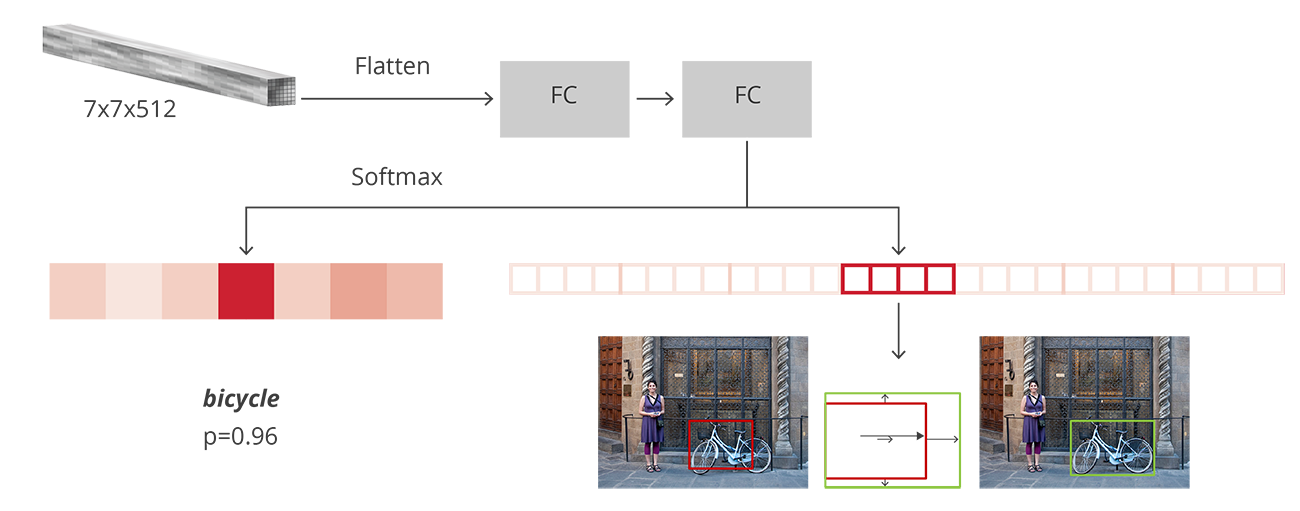
\includegraphics[width=\textwidth]{rcnn-architecture}
	\caption{Example of classification flow in the \gls{rcnn} classifying a bicycle and regressing a bounding box \citep{Rey2018}}
	\label{fig:rcnn_ex}
\end{figure}

%\graphicspath{{figures/implementation/}}
\chapter{Implementation}\label{ch:implementation}\glsresetall

In this chapter the development work carried out throughout this project is documented. Each section contains some theoretical descriptions of the methods used as well as descriptions of the actual implementational work. 

\graphicspath{{figures/results/}}
\chapter{Results}
The results presented are both training and testing results from the two solutions. Both the image classification and the multi-class object detection are trained and tested on the 60 seconds video with three zebrafish.

The solutions are trained on annotated data of 411 different occlusions in total and a similar amount annotated occurrences of \textit{no occlusions}.

\section{Image Classification}
The image classification solution is trained for 15 epochs, the results are shown in \autoref{fig:img_class-15ep}
\begin{figure}[H]
	\centering
	\begin{subfigure}{0.48\textwidth}
		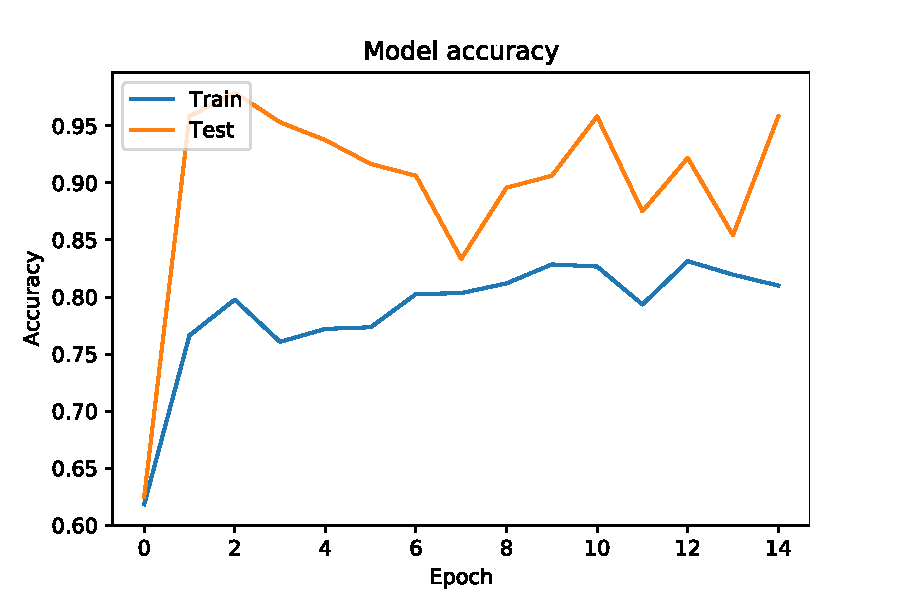
\includegraphics[width=\textwidth]{model_acc_15epoch}
		\caption{The image classification accuracy for both training and testing}
		\label{fig:img_acc-15}
	\end{subfigure}
	\begin{subfigure}{0.48\textwidth}
		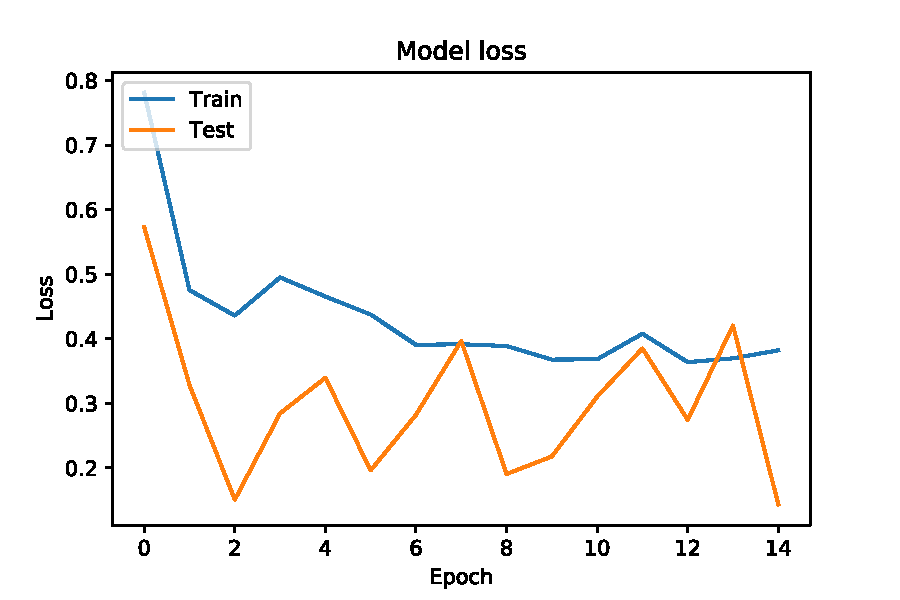
\includegraphics[width=\textwidth]{model_loss_15epoch}
		\caption{The image classification loss for both training and testing}
		\label{fig:img_loss-15}
	\end{subfigure}
\caption{Model accuracy and loss when trained for 15 epochs}
\label{fig:img_class-15ep}
\end{figure}

As shown in \autoref{fig:img_class-15ep} the training accuracy is lower than the testing accuracy, however, the training graph is in both functions more stable and seems closer to converging than the testing graph. Meanwhile, the training loss is  higher than the test loss as well.

In general, the model is still unstable and needs more training for converging.

\autoref{tab:img_class_15ep} also shows that the test results are better than the training.
\begin{table}[H]
	\centering
	\caption{End results achieved with 15 epochs.}
	\begin{tabular}{|l|l|}
		\hline
		Training Loss                	& 0.4841 			\\\rowcolor{lightGrey}\hline
		Training Accuracy       	    & 0.7738 			\\ \hline
		Testing Loss     				& 0.2487 			\\\rowcolor{lightGrey}\hline
		Testing Accuracy 				& 0.9318			\\ \hline
	\end{tabular}
\label{tab:img_class_15ep}
\end{table}

The image detection model is also trained for 100 epochs, the results of this is shown in \autoref{fig:img_class-100ep} and \autoref{tab:img_class_100ep}.
\begin{figure}[H]
	\centering
	\begin{subfigure}{0.48\textwidth}
		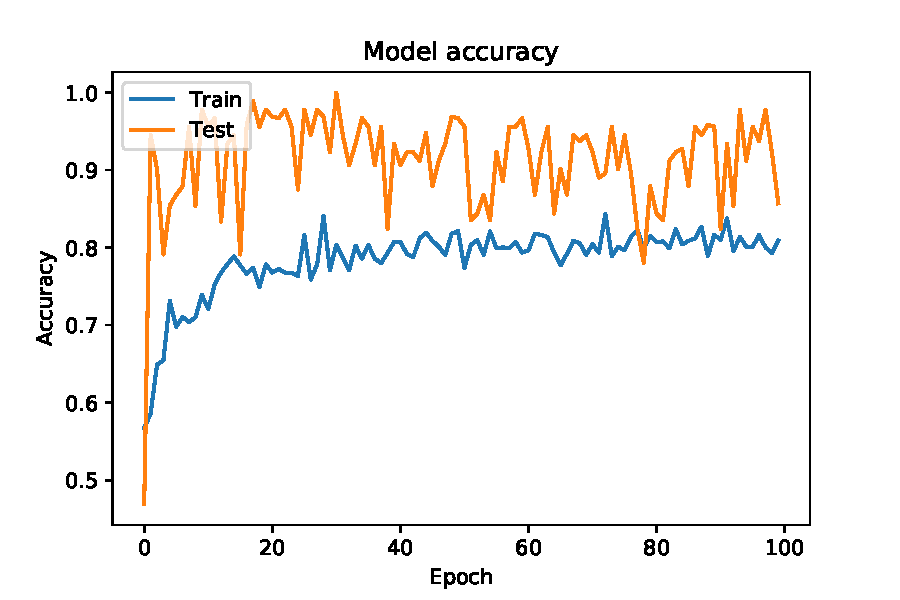
\includegraphics[width=\textwidth]{model_acc_100epoch}
		\caption{The image classification accuracy for both training and testing}
		\label{fig:img_acc-100}
	\end{subfigure}
	\begin{subfigure}{0.48\textwidth}
		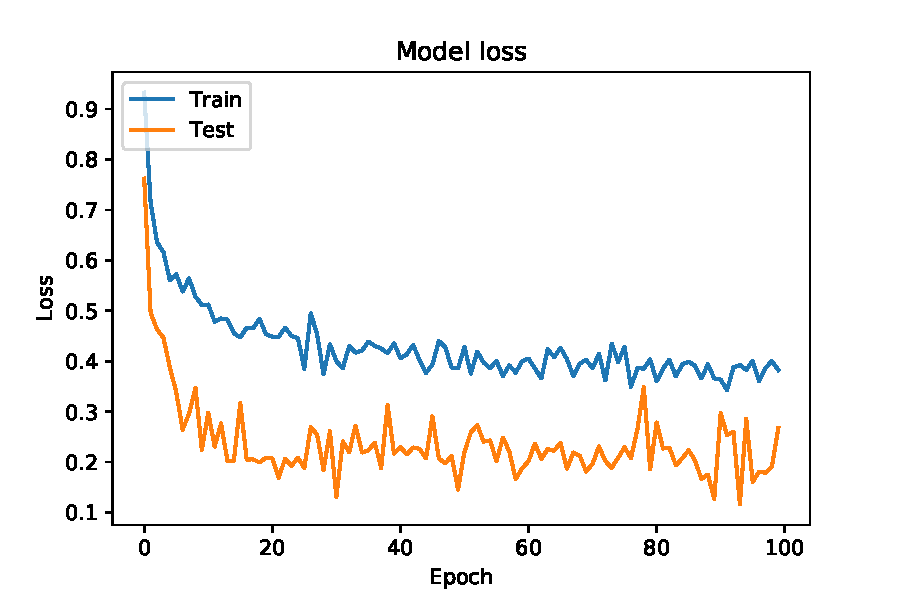
\includegraphics[width=\textwidth]{model_loss_100epoch}
		\caption{The image classification loss for both training and testing}
		\label{fig:img_loss-100}
	\end{subfigure}
\caption{Model accuracy and loss when trained for 100 epochs}
\label{fig:img_class-100ep}
\end{figure}
There is still a high amount of instability, but in general the test results are better than the training. It has tendencies towards converging, but it is uncertain due to the instability.

\begin{table}[H]
	\centering
	\caption{End results achieved with 100 epochs.}
	\begin{tabular}{|l|r|}
		\hline
		Training Loss            		& 0.3831	\\ \rowcolor{lightGrey}\hline
		Training Accuracy        	    & 0.8075 	\\ \hline
		Testing Loss     				& 0.2680	\\ \rowcolor{lightGrey}\hline
		Testing Accuracy 				& 0.8571	\\ \hline
	\end{tabular}
	\label{tab:img_class_100ep}
\end{table}

\section{Object Detection}
The Faster \gls{rcnn} object detection model is trained with a split of $85\%$ for training and $15\%$ for testing.

\subsection{Training}
Training is done at 42 and 152 epochs, as these points had an automatic stop. When training, the best performing weights are saved.

\subsubsection{42 Epochs}
After the object detection model has been trained for 42 epochs, the training accuracy is as shown in the following figures:
\begin{figure}[H]
	\centering
	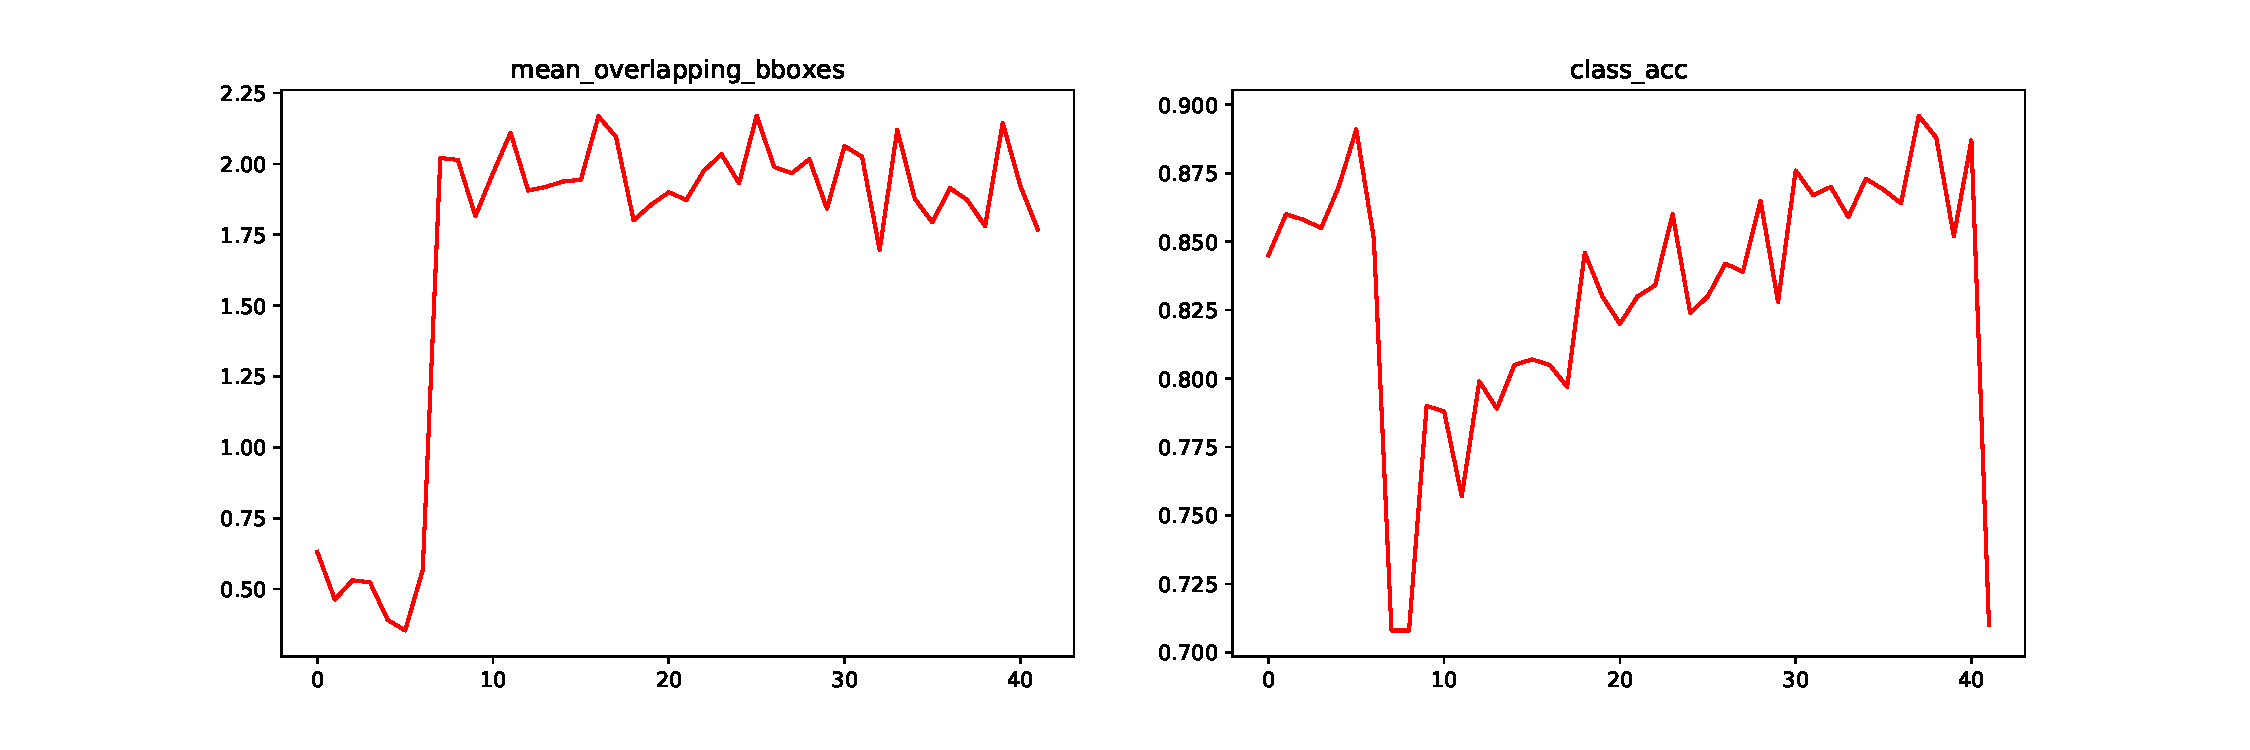
\includegraphics[width=\textwidth]{acc-42}
	\caption{Mean of overlapping bounding boxes of ground truth and classification accuracy}
	\label{fig:acc-42}
\end{figure}
\autoref{fig:acc-42} shows the mean overlapping bounding boxes of the ground truth bounding box, and the classification accuracy of the \gls{rcnn} classifier.

\begin{figure}[H]
	\centering
	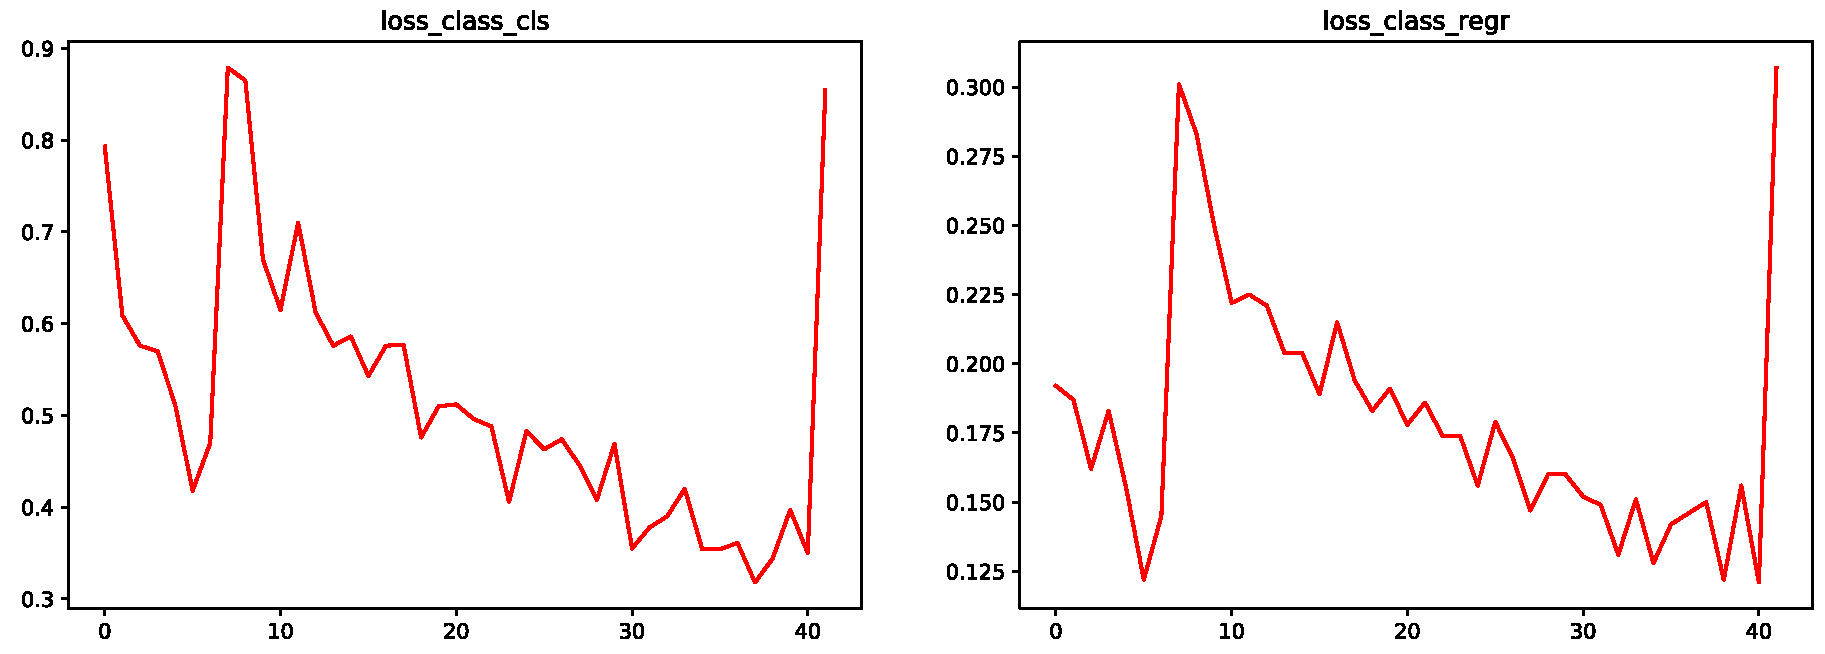
\includegraphics[width=\textwidth]{loss_class-42}
	\caption{Loss in classification and general bounding box regression}
	\label{fig:loss_class-42}
\end{figure}
\autoref{fig:loss_class-42} shows the loss in the \gls{rcnn} classifier and bounding box regression.

\begin{figure}[H]
	\centering
	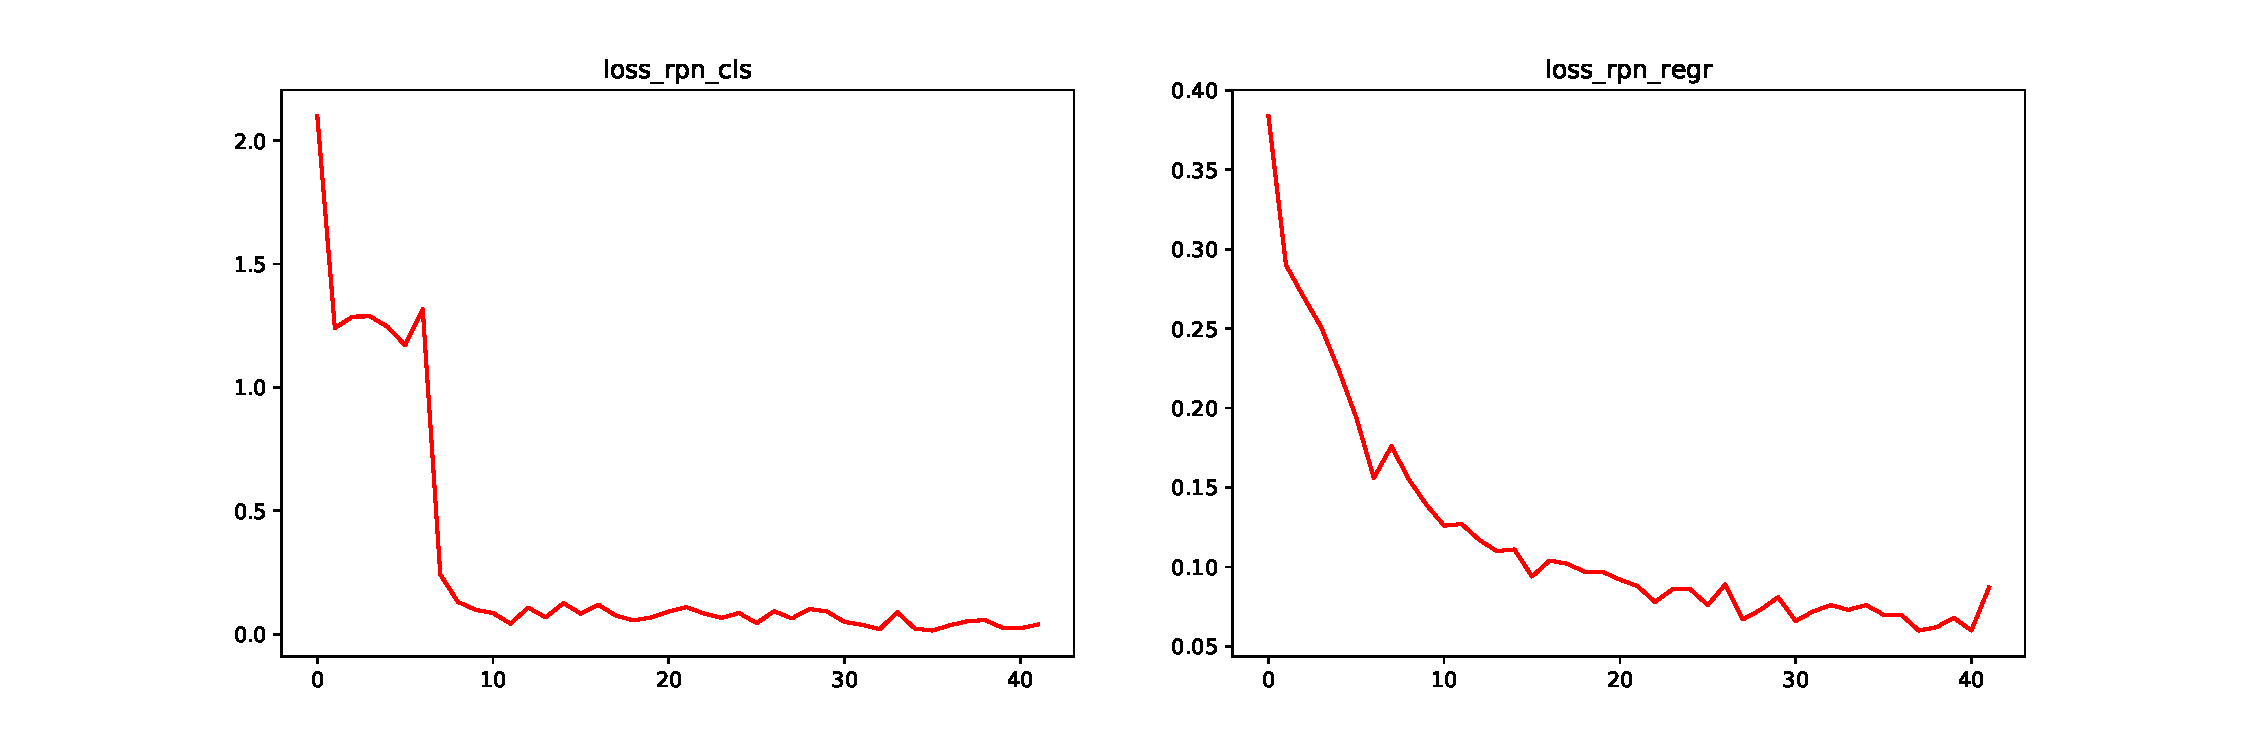
\includegraphics[width=\textwidth]{loss_rpn-42}
	\caption{Loss in the \gls{rpn} classification and general bounding box regression}
	\label{fig:loss_rpn-42}
\end{figure}
\autoref{fig:loss_rpn-42} shows the loss in the \gls{rpn} classifier and bounding box regression.

\begin{figure}[H]
	\centering
	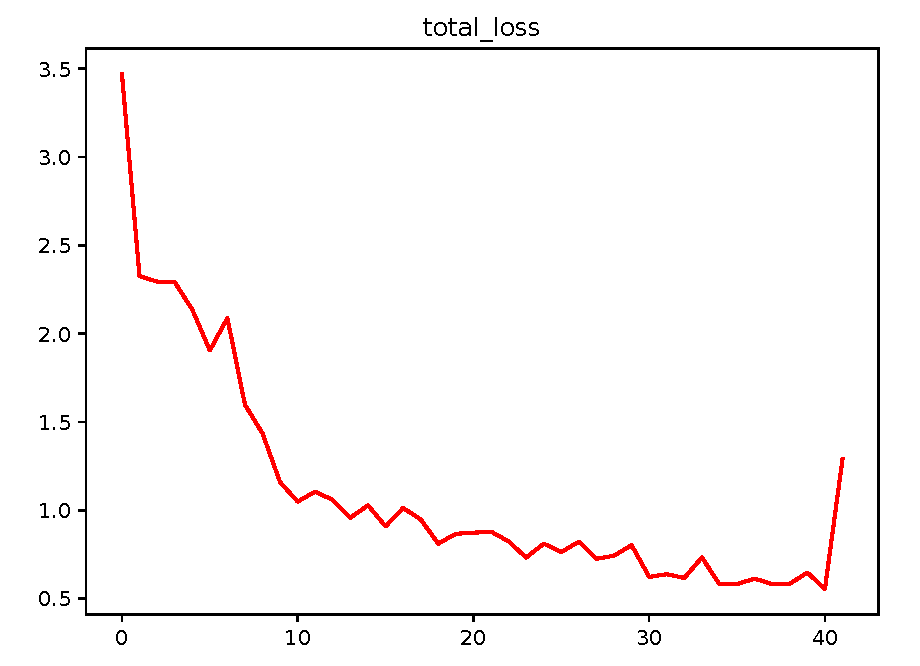
\includegraphics[width=0.7\textwidth]{total_loss-42}
	\caption{Total loss of the entire model}
	\label{fig:total_loss-42}
\end{figure}
\autoref{fig:total_loss-42} shows the total loss of the model during training. The \gls{rcnn} classification and regression steps show signs of instability, which is seen in the loss and the accuracy of both overlapping bounding boxes and the classification accuracy.

When testing with these results, the test was stopped due to poor performance.

\subsubsection{152 Epochs}
After the object detection model has been trained for 152 epochs, the training accuracy is as shown in the following figures:
\begin{figure}[H]
	\centering
	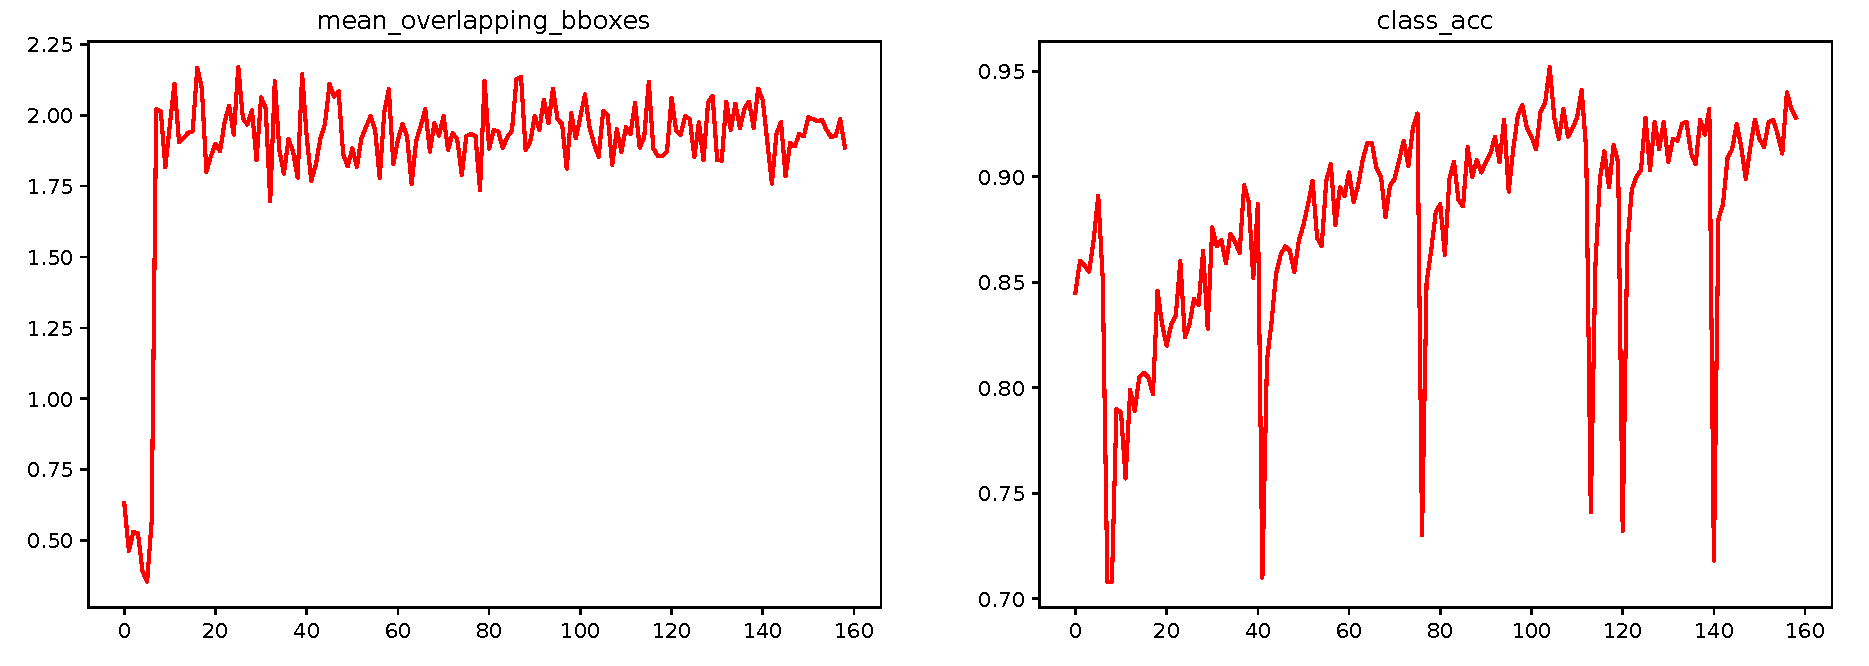
\includegraphics[width=\textwidth]{acc-152}
	\caption{Mean of overlapping bounding boxes of ground truth and classification accuracy}
	\label{fig:acc-152}
\end{figure}
\autoref{fig:acc-152} shows the mean overlapping bounding boxes of the ground truth bounding box, and the classification accuracy of the \gls{rcnn} classifier.

\begin{figure}[H]
	\centering
	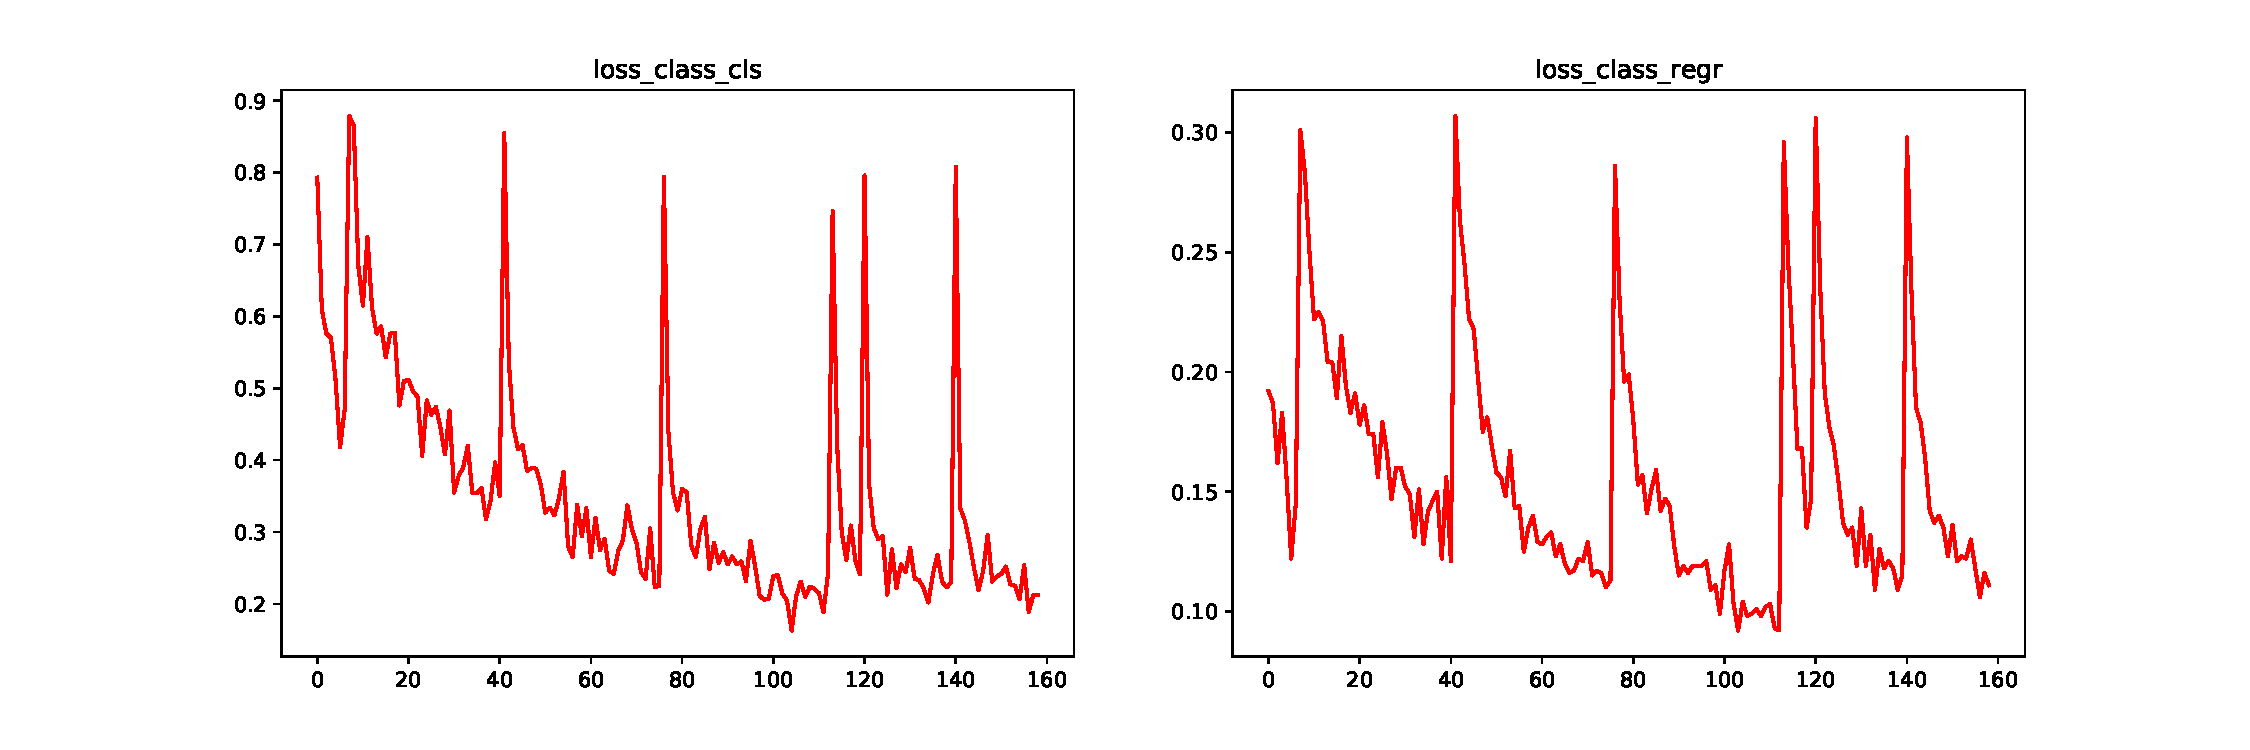
\includegraphics[width=\textwidth]{loss_class-152}
	\caption{Loss in classification and general bounding box regression}
	\label{fig:loss_class-152}
\end{figure}
\autoref{fig:loss_class-152} shows the loss in the \gls{rcnn} classifier and bounding box regression.

\begin{figure}[H]
	\centering
	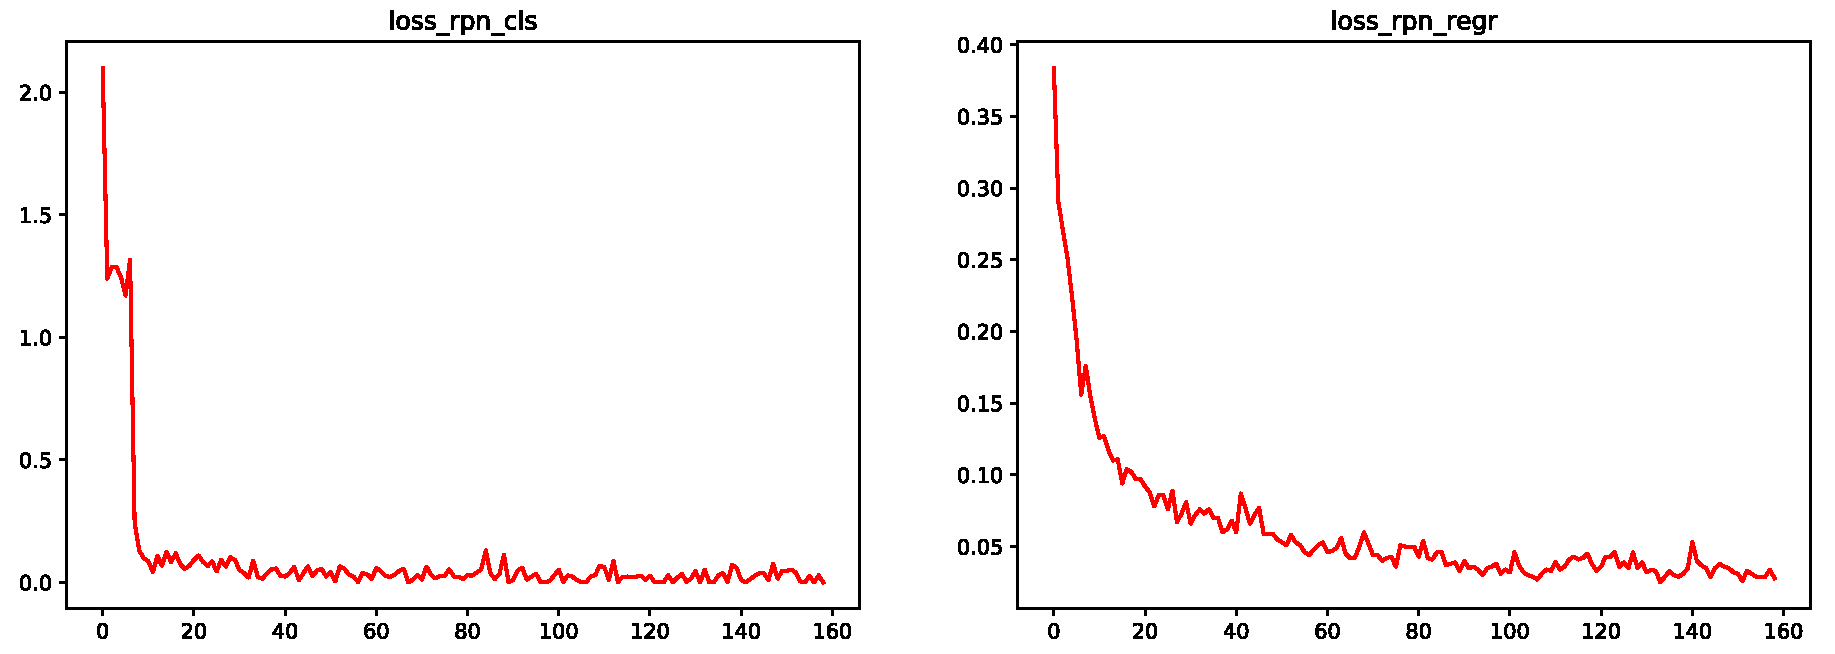
\includegraphics[width=\textwidth]{loss_rpn-152}
	\caption{Loss in the \gls{rpn} classification and general bounding box regression}
	\label{fig:loss_rpn-152}
\end{figure}
\autoref{fig:loss_rpn-152} shows the loss in the \gls{rpn} classifier and bounding box regression.

\begin{figure}[H]
	\centering
	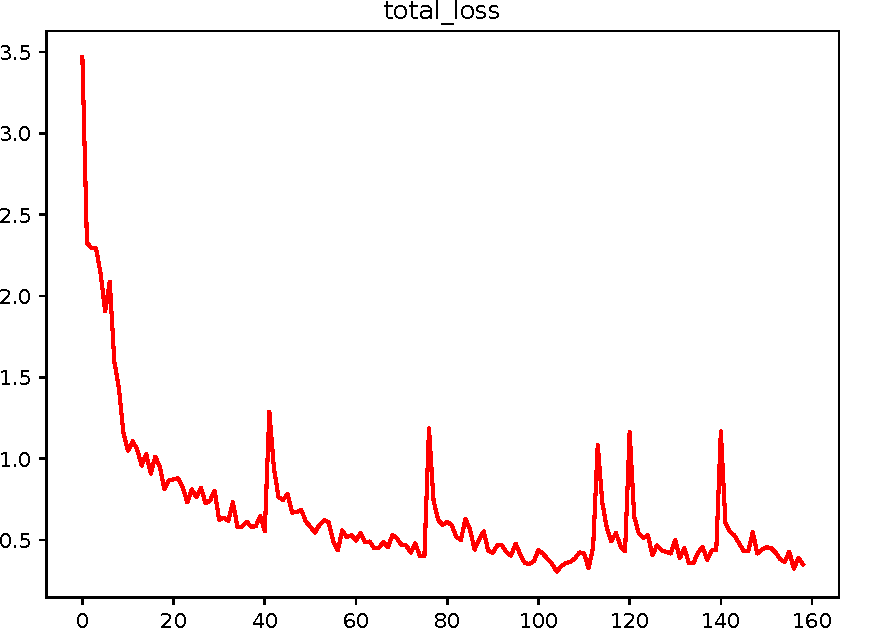
\includegraphics[width=0.7\textwidth]{total_loss-152}
	\caption{Total loss of the entire model}
	\label{fig:total_loss-152}
\end{figure}
\autoref{fig:total_loss-152} shows the total loss of the model during training. There are still signs of instability and again especially in the \gls{rcnn} classification and regression. However, there are signs towards the model converging.

\subsection{Testing}
The training and testing split is $85\%$ for training and $15\%$ for testing. With this split the solution reaches a \gls{map} of $66.8\%$.

\autoref{fig:T-det}, \ref{fig:not-det}, and \ref{fig:no-occl-det} show plots of predictions of three random testing frames, with predictions and bounding box regressions. The predictions and the accuracy is written in the image caption. Only detections with a confidence above $70\%$ are accepted.\\

\autoref{tab:class-pred} shows that the average precision is very different between classes, ranging from $34.4\%$ to $ 100\% $.
\begin{table}[H]
	\centering
	\caption{Average precisions of the different occlusion types}
	\label{tab:class-pred}
	\begin{tabular}{lr}
		\textbf{Occlusion Type} & \textbf{Average Precision} \\\rowcolor{lightGrey}\hline
		T Shape                 & $ 74.6\% $                     \\
		V Shape                 & $ 53.9\% $                    \\\rowcolor{lightGrey}
		On Top                  & $ 100\% $                      \\
		Cross                   & $ 78.2\% $                     \\\rowcolor{lightGrey}
		Elongation              & $ 91.9\% $                     \\
		Other                   & $ 37.6\% $                     \\\rowcolor{lightGrey}
		No Occlusion            & $ 34.6\% $                    
	\end{tabular}
\end{table}



\autoref{fig:T-det} shows two zebrafish creating a T-shape occlusion, which is detected with a confidence of $91.37\%$ and single zebrafish detected as no occlusion with a confidence of $99.48\%$.
\begin{figure}[H]
	\centering
	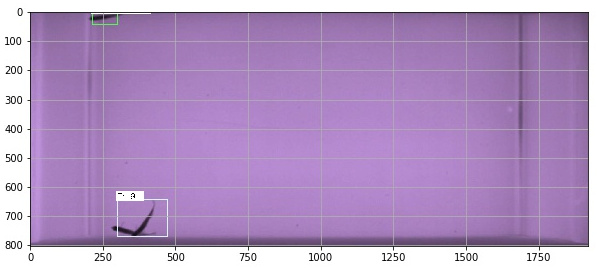
\includegraphics[width=\textwidth]{prediction-frame596}
	\caption{Detection of the T-shape is with a confidence of $91.37\%$ and of no occlusion with $99.48\%$}
	\label{fig:T-det}
\end{figure}

\autoref{fig:not-det} shows a crossing occlusion which is not being detected and a single zebrafish detected as no occlusion with a confidence of $99.43\%$.
\begin{figure}[H]
	\centering
	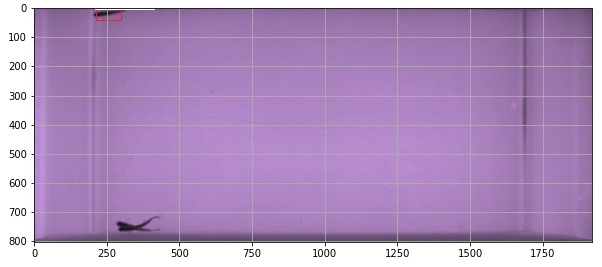
\includegraphics[width=\textwidth]{prediction-frame601}
	\caption{Only detection of no occlusion with confidence of $99.43\%$}
	\label{fig:not-det}
\end{figure}

\autoref{fig:no-occl-det} shows three zebrafish with no occlusions occurring in the image, but only two of them are detected as no occlusions, with confidences of $99.48\%$ and $98.73\%$. The last zebrafish does not have a detection confidence higher than $70\%$ and is therefore ignored.
\begin{figure}[H]
	\centering
	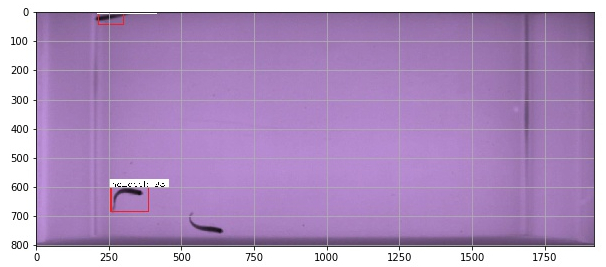
\includegraphics[width=\textwidth]{prediction-frame1092}
	\caption{Two detections of no occlusions with confidence of $99.48\%$ and $98.73\%$}
	\label{fig:no-occl-det}
\end{figure}
\chapter{Evaluation}

\chapter{Conclusion}\label{ch:conclusion}\glsresetall
Throughout the project, the work has been aimed at finding an answer to the problem statement:

\textit{How can a zebrafish occlusion detection solution be implemented in order to potentially optimise zebrafish tracking?}\\

In order to be able to detect zebrafish occlusions two different solutions is made. To be able to cater to different occlusion handling approaches a more simple image classification occlusion detection was developed, as to enable a user to solve the occlusions occurring during a tracking process. 

If occlusions need solving before any tracking is done, an object detection is implemented to locate and classify the occlusions in an image.\\

The image classification achieves a validation accuracy of $93\%$ when trained for 15 epochs, but shows a lot of instability which can point towards a "lucky hit". When training for longer, no convergence is achieved which may point towards the need of more data or tweaking of hyper parameters.\\

The object detection achieves a \gls{map} of $66.8\%$, and is able to locate both occlusions and single zebrafish as \textit{no occlusion}. It is not able to detect all types of occlusions with some classes having a rather low average precision in testing pointing towards the need of more data to increase performance.
\chapter{Future Work}


% For use if report is split up in parts
\bookmarksetup{startatroot}% Goto root of Table of Contents
\addtocontents{toc}{\bigskip}% Add space before next item in Table of Contents

% Appearance of the bibliography
\iflanguage{english}{%
\bibliographystyle{setup/plainnat_en}%
}{%
\bibliographystyle{setup/plainnat_dk}%
}
\label{LastPage}


\bibliography{bib/VGIS10}
\label{bib:mybiblio}




%\setlength{\chapnumb}{2cm} % Ændrer længden på stregen under kapiteloverskriften så den passer til bilag
\appendix % Start of appendix
\addtocontents{toc}{\protect\setcounter{tocdepth}{0}}
%\graphicspath{{figures/appendix/}}
\input{chapters/appendices/guitar_meas}
\input{chapters/appendices/pedal_meas}
\input{chapters/appendices/setup_code}
\input{chapters/appendices/signal_to_noise.tex}
\input{chapters/appendices/echo_meas}
\input{chapters/appendices/flanger_meas}
\input{chapters/appendices/reverb_meas}
\input{chapters/appendices/eq_meas}

%%\input{chapters/appendices/code}

\end{document}
